% ============================================================
% NLP for Structured HAZOP Reasoning --- Weekly Research Log
%
% MAINTENANCE NOTE (read this before editing):
%   - Each week gets its own file: weeks/weekNN.tex
%   - A new week is added to the document by (1) creating
%     weeks/weekNN.tex following the pattern of weeks/week01.tex,
%     and (2) adding one \input{weeks/weekNN} line below, in order.
%   - Each week file must start with
%       \section[<short title>]{<full title>}
%     The optional short title is what appears in the running
%     header and the table of contents, so keep it under ~50
%     characters or it will run into the left-hand header.
%   - Never delete or renumber a previous week's \input line.
%   - Shared bibliography lives in references.bib; append new
%     entries there, do not create per-week bibliographies.
%   - Shared TikZ node styles, tcolorbox callouts and the
%     \yes/\prt/\no capability marks are defined in this preamble
%     so that every week's diagrams look the same. Add new shared
%     styles here, not inside a week file.
%   - Recompile with: pdflatex main && bibtex main &&
%     pdflatex main && pdflatex main   (two pdflatex passes after
%     bibtex to resolve cross-references and the bibliography).
% ============================================================

% This is a formal report: each major research stage is a chapter.
\documentclass[10pt,a4paper]{report}

\usepackage[a4paper,margin=0.8in,headheight=14pt,headsep=10pt]{geometry}
\usepackage[T1]{fontenc}
\usepackage{lmodern}
\usepackage{amsmath}
\usepackage{amssymb}
\usepackage{microtype}
\usepackage{enumitem}
\usepackage{etoolbox}
\usepackage{booktabs}
\usepackage{tabularx}
\usepackage{xcolor}
\usepackage[most]{tcolorbox}
\usepackage{tikz}
\usetikzlibrary{arrows.meta,positioning,fit,backgrounds,calc}
\usepackage[font=small,labelfont=bf,skip=8pt]{caption}
\usepackage[english]{babel}
\usepackage{titlesec}
\usepackage{fancyhdr}
\usepackage{hyperref} % load last

\hypersetup{
  colorlinks=true,
  linkcolor=black,
  citecolor=black,
  urlcolor=blue,
  pdftitle={NLP for Structured HAZOP Reasoning},
  pdfauthor={Prasangeet Dongre}
}

% ------------------------------------------------------------
% Shared palette
% ------------------------------------------------------------
\definecolor{hzblue}{HTML}{1F4E79}
\definecolor{hzbluebg}{HTML}{DCE6F1}
\definecolor{hzgray}{HTML}{4B5563}
\definecolor{hzgraybg}{HTML}{F2F3F5}
\definecolor{hzgreen}{HTML}{166534}
\definecolor{hzgreenbg}{HTML}{DFF3E3}
\definecolor{hzamber}{HTML}{92590B}
\definecolor{hzamberbg}{HTML}{FBF0D9}
\definecolor{hzred}{HTML}{8C1D1D}
\definecolor{hzredbg}{HTML}{FBE4E4}

% ------------------------------------------------------------
% Sectioning and spacing --- tightened a little, not squeezed
% ------------------------------------------------------------
\titleformat{\chapter}{\normalfont\Large\bfseries\color{hzblue}}{Week~\thechapter}{0.8em}{}
\titleformat{\section}{\normalfont\large\bfseries\color{hzblue}}{\thesection}{0.8em}{}
\titleformat{\subsection}{\normalfont\normalsize\bfseries}{\thesubsection}{0.8em}{}
\titleformat{\subsubsection}{\normalfont\small\bfseries\itshape}{\thesubsubsection}{0.8em}{}
\titlespacing*{\chapter}{0pt}{0pt}{1.5ex}
\titlespacing*{\section}{0pt}{1.8ex plus .3ex minus .2ex}{0.8ex plus .2ex}
\titlespacing*{\subsection}{0pt}{1.4ex plus .2ex minus .2ex}{0.5ex plus .1ex}
\titlespacing*{\subsubsection}{0pt}{1.1ex plus .2ex minus .2ex}{0.4ex plus .1ex}
\titlespacing*{\paragraph}{0pt}{1ex plus .2ex}{0.6em}

\setlist{topsep=4pt,itemsep=3pt,parsep=0pt,partopsep=0pt,leftmargin=1.8em}
\setlength{\abovedisplayskip}{4pt}
\setlength{\belowdisplayskip}{4pt}
\setlength{\parindent}{1em}
\setlength{\parskip}{0pt}
\apptocmd{\thebibliography}{\setlength{\itemsep}{3pt}\setlength{\parsep}{0pt}}{}{}

\setcounter{secnumdepth}{3} % number subsubsections too
\setcounter{tocdepth}{3}    % ...and list them, but keep \paragraph out of the ToC

% ------------------------------------------------------------
% Running head. \leftmark is fed by \sectionmark, which in the
% article class receives the optional (short) argument of \section.
% ------------------------------------------------------------
\pagestyle{fancy}
\fancyhf{}
\fancyhead[L]{\small\color{hzgray}NLP for Structured HAZOP Reasoning}
\fancyhead[R]{\small\color{hzgray}\nouppercase{\leftmark}}
\fancyfoot[C]{\small\thepage}
\renewcommand{\headrulewidth}{0.4pt}

% ------------------------------------------------------------
% Shared diagram styles (used by every week's figures)
% ------------------------------------------------------------
\tikzset{
  % a node in a causal chain that the worksheet does record
  ev/.style={draw=hzblue,fill=hzbluebg,rounded corners=2pt,align=center,
             font=\scriptsize,text width=19mm,minimum height=9.5mm,inner sep=2pt},
  % an intermediate event the flat worksheet drops
  interev/.style={ev,fill=white,draw=hzgray,densely dashed},
  % a safeguard
  sg/.style={draw=hzgreen,fill=hzgreenbg,rounded corners=2pt,align=center,
             font=\scriptsize,text width=20mm,inner sep=2pt},
  % an input / artefact box in a pipeline figure
  art/.style={draw=hzgray,fill=hzgraybg,rounded corners=2pt,align=center,
              font=\scriptsize,text width=21mm,minimum height=9mm,inner sep=2pt},
  % a processing step in a pipeline figure
  proc/.style={draw=hzblue,fill=hzbluebg,rounded corners=2pt,align=center,
               font=\scriptsize,text width=21mm,minimum height=9mm,inner sep=2pt},
  % the outcome of a pipeline
  outc/.style={draw=hzamber,fill=hzamberbg,rounded corners=2pt,align=center,
               font=\scriptsize,text width=21mm,minimum height=9mm,inner sep=2pt},
  ar/.style={-{Latex[length=1.8mm,width=1.5mm]},hzblue,semithick},
  sgar/.style={-{Latex[length=1.6mm,width=1.3mm]},hzgreen,densely dashed,thin},
  tag/.style={font=\scriptsize\itshape,text=hzgray,align=center,inner sep=1pt},
  lane/.style={font=\scriptsize\bfseries,text=hzblue,align=right,inner sep=1pt},
}

% ------------------------------------------------------------
% Shared callout boxes
% ------------------------------------------------------------
% A hard constraint the write-up must respect from now on.
\newtcolorbox{constraint}[1][]{enhanced,breakable,
  colback=hzredbg,colframe=hzred,boxrule=0.5pt,
  fonttitle=\bfseries\small,coltitle=white,colbacktitle=hzred,
  title={#1},left=6pt,right=6pt,top=4pt,bottom=4pt,
  before skip=7pt,after skip=7pt}
% A claim that is still provisional / not yet defensible.
\newtcolorbox{provisional}[1][]{enhanced,breakable,
  colback=hzamberbg,colframe=hzamber,boxrule=0.5pt,
  fonttitle=\bfseries\small,coltitle=white,colbacktitle=hzamber,
  title={#1},left=6pt,right=6pt,top=4pt,bottom=4pt,
  before skip=7pt,after skip=7pt}
% Week-at-a-glance summary.
\newtcolorbox{glance}[1][]{enhanced,breakable,
  colback=hzbluebg,colframe=hzblue,boxrule=0.5pt,
  fonttitle=\bfseries\small,coltitle=white,colbacktitle=hzblue,
  title={#1},left=6pt,right=6pt,top=4pt,bottom=4pt,
  before skip=7pt,after skip=7pt}

% Capability-matrix marks
\newcommand{\yes}{\textcolor{hzgreen}{$\checkmark$}}
\newcommand{\prt}{\textcolor{hzamber}{$\sim$}}
\newcommand{\no}{\textcolor{hzred}{$\times$}}

\title{NLP for Structured HAZOP Reasoning\\[0.4em]
\large Research Report}
\author{Prasangeet Dongre\\
\small Roll No.: B23CH1033\\
\small Department of Chemical Engineering\\
\small Advisor: Dr. Santhosh Kumar Varanasi}
\date{\today}

\begin{document}

\maketitle

\begin{abstract}
Hazard and Operability Study (HAZOP) reports encode process-safety knowledge
in a structured but predominantly tabular form. This report examines whether
natural-language processing and large language models can support reasoning
over that knowledge rather than only extracting labels from report text. A
survey of HAZOP automation literature is combined with a detailed analysis of
an ontology-based HAZOP reasoner. The review shows that causal, multi-step,
branching inference is already possible when process and safety knowledge are
manually encoded. The remaining research question is therefore narrower:
whether causal knowledge can be reconstructed from unstructured historical
HAZOP reports and then constrained or validated using structured reasoning.
This distinction provides a more defensible foundation for future system
design and evaluation.
\end{abstract}

\noindent\textbf{Keywords:} HAZOP; process safety; natural-language processing;
knowledge graphs; ontology reasoning; causal inference; large language models

\clearpage
\pagenumbering{roman}
\tableofcontents
\listoffigures
\clearpage
\pagenumbering{arabic}

% Main paper sections are maintained in separate source files.
% ============================================================
% Week 01 section --- NLP for Structured HAZOP Reasoning
%
% Structure of a week file:
%   \section[<short title, for header + ToC>]{<full title>}
%   then \subsection blocks. Shared TikZ styles (ev, interev,
%   sg, art, proc, outc, ar, sgar, tag, lane), the callout
%   environments (glance, constraint, provisional) and the
%   \yes/\prt/\no marks all come from main.tex's preamble.
%
% Bibliography entries are in references.bib; several entries
% are marked VERIFY there and must be checked against the
% original source before final submission.
% ============================================================

% The optional short title feeds both the ToC and the running header.
\chapter[Background and Literature Survey]{Background, Literature Survey, and Research Framing}

This section establishes HAZOP fundamentals, defines the project framing, and
surveys prior work on automated HAZOP analysis. The review shows that the
research problem must be stated more narrowly than the initial framing.

\section{Project Motivation}
HAZOP (Hazard and Operability Study) is a structured method for identifying hazards and operability issues in chemical processes. Reports are typically authored manually and stored as tabular worksheets. This project investigates whether NLP/LLM methods can support structured reasoning over the knowledge contained in HAZOP reports, rather than treating HAZOP text purely as a source for information extraction.

\section{Fundamentals of HAZOP}
\begin{itemize}
  \item \textbf{Node}: a defined section of a process (e.g., a vessel, a line between two points) selected for study.
  \item \textbf{Parameter}: a process variable examined at a node (e.g., flow, temperature, pressure, level).
  \item \textbf{Guide word}: a standardized qualifier (e.g., NO, MORE, LESS, REVERSE) combined with a parameter to systematically generate deviations.
  \item \textbf{Deviation}: a guide word applied to a parameter (e.g., ``MORE temperature'').
  \item \textbf{Cause}: a condition or event that could produce the deviation.
  \item \textbf{Consequence}: the potential outcome if the deviation occurs and is not mitigated.
  \item \textbf{Safeguard}: an existing protection (alarm, interlock, relief device, procedure) that reduces likelihood or severity.
\end{itemize}

\section{HAZOP as a Reasoning Structure}
A HAZOP worksheet presents Cause, Deviation, Consequence, and Safeguard as flat table columns. This is a presentational simplification: the underlying process-safety knowledge can involve intermediate events, multiple contributing causes, branching consequences, and multiple safeguards acting at different points in a chain. Figure~\ref{fig:flat-vs-chain} contrasts the two views for a single worksheet row.

\begin{figure}[htbp]
\centering

% ---------- panel (a): what the worksheet records ----------
{\small
\begin{tabular}{@{}llll@{}}
\toprule
\textbf{Deviation} & \textbf{Cause} & \textbf{Consequence} & \textbf{Safeguards} \\
\midrule
MORE temperature & Cooling pump failure & Reactor overpressure & TAH; PSV; ESD \\
\bottomrule
\end{tabular}}

\vspace{0.4em}
{\small (a) the worksheet row: four flat fields, no ordering between them}

\vspace{1.4em}

% ---------- panel (b): the underlying causal structure ----------
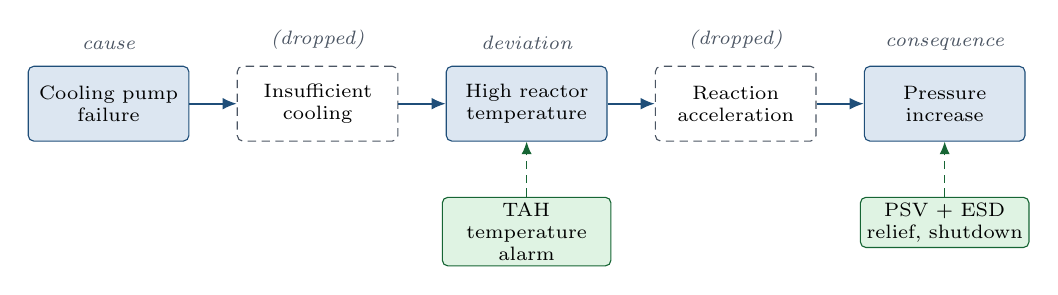
\begin{tikzpicture}[node distance=5.5mm and 6mm]
  \node[ev]                (n1) {Cooling pump\\ failure};
  \node[interev,right=of n1] (n2) {Insufficient\\ cooling};
  \node[ev,right=of n2]      (n3) {High reactor\\ temperature};
  \node[interev,right=of n3] (n4) {Reaction\\ acceleration};
  \node[ev,right=of n4]      (n5) {Pressure\\ increase};
  \foreach \a/\b in {n1/n2,n2/n3,n3/n4,n4/n5} \draw[ar] (\a) -- (\b);

  % worksheet column roles
  \node[tag,above=1.6mm of n1] {cause};
  \node[tag,above=1.6mm of n2] {(dropped)};
  \node[tag,above=1.6mm of n3] {deviation};
  \node[tag,above=1.6mm of n4] {(dropped)};
  \node[tag,above=1.6mm of n5] {consequence};

  % safeguards act at specific points, not on the row as a whole
  \node[sg,below=7mm of n3] (s1) {TAH\\ temperature alarm};
  \node[sg,below=7mm of n5] (s2) {PSV + ESD\\ relief, shutdown};
  \draw[sgar] (s1) -- (n3);
  \draw[sgar] (s2) -- (n5);
\end{tikzpicture}

\vspace{0.4em}
{\small (b) the underlying chain: dashed boxes are intermediate events the\\ worksheet has no column for; safeguards attach to specific events}

\caption[Flat worksheet row versus the underlying causal chain]{The same
hazard scenario as a flat worksheet row (a) and as a causal chain with
event-specific safeguards (b). The flattening loses the intermediate events
and the attachment point of each safeguard --- which is what makes the row
hard to reason over automatically.}
\label{fig:flat-vs-chain}
\end{figure}

Representing this as a graph rather than a table is \emph{not} itself a novel observation --- it is a modeling choice that recurs across the digraph, ontology, and knowledge-graph literature (Categories A, B, D below). What varies across papers is not whether a graph representation is used, but how the graph is populated (manual encoding vs.\ text extraction) and what operations are performed on it (traversal vs.\ learned reasoning vs.\ free generation).

\section{Initial Project Objective (Provisional)}
Initially hypothesized objective: extract causal structure from unstructured historical HAZOP report text and represent it as a graph capable of supporting inference of missing causes, consequences, or safeguards. This objective is recorded here for continuity only --- it predates the literature findings below and should not be treated as validated or final.

\section{Literature Survey}
The initial literature set was organized into five provisional categories. Figure~\ref{fig:lanes} shows what distinguishes them in practice: where each family gets its structure from, and what it then does with it.

\paragraph{A. Classical model-based / expert-system HAZOP.}
Vaidhyanathan \& Venkatasubramanian \cite{vaidhyanathan1995digraph,vaidhyanathan1996experience}; Rahman et al., ExpHAZOP+ \cite{rahman2009exphazop}; Rodr{\'i}guez \& de la Mata, D-higraphs \cite{rodriguez2012dhigraphs}; Taylor \cite{taylor2017automated}. These operate on hand-built process models rather than natural-language text; reasoning proceeds via digraph traversal or rule-chaining over a manually constructed representation.

\paragraph{B. Ontology-based causal reasoning.}
Aziz et al.\ \cite{aziz2019ontology}; Single et al.\ \cite{single2020ontologyhazop}. Causal relationships between HAZOP concepts are explicitly encoded in an ontology and processed by a semantic reasoner.

\paragraph{C. NLP/ML applied to HAZOP text.}
Feng et al.\ (2021, NLP in HAZOP reports) \cite{feng2021nlphazop}; Wang et al.\ (2021, active learning/text mining) \cite{wang2021activelearning}; Wang \& Gu (2022, data mining) \cite{wanggu2022datamining}; Ekramipooya et al.\ \cite{ekramipooya2023deviation,ekramipooya2024recommendation}. These extract or classify information from HAZOP text (entity recognition, deviation-category prediction, recommendation clustering) without constructing or reasoning over an explicit causal graph.

\paragraph{D. Knowledge graphs and structured HAZOP reasoning.}
Mao et al.\ \cite{mao2020processsafetykg}; Feng et al.\ (2021, causal ontology description model) \cite{feng2021hazopcausal}; Wang et al.\ (2022, ISKG/HAINEX) \cite{wang2022iskghainex}; Li \& Zhao (2024) \cite{lizhao2024constructing}; Li \& Zhao (2025, HAZOPCT) \cite{lizhao2025hazopct}. These construct HAZOP knowledge graphs, in several cases via NLP-based entity extraction from text, and apply graph-based reasoning methods over the resulting structure.

\paragraph{E. LLM-based HAZOP generation.}
Lee et al.\ \cite{lee2026llmhazop}. Multimodal LLMs generate complete HAZOP worksheets end-to-end from a P\&ID and a standardized prompt, without an intermediate structured representation.

These categories are provisional and may be revised as the survey deepens.

\begin{figure}[htbp]
\centering
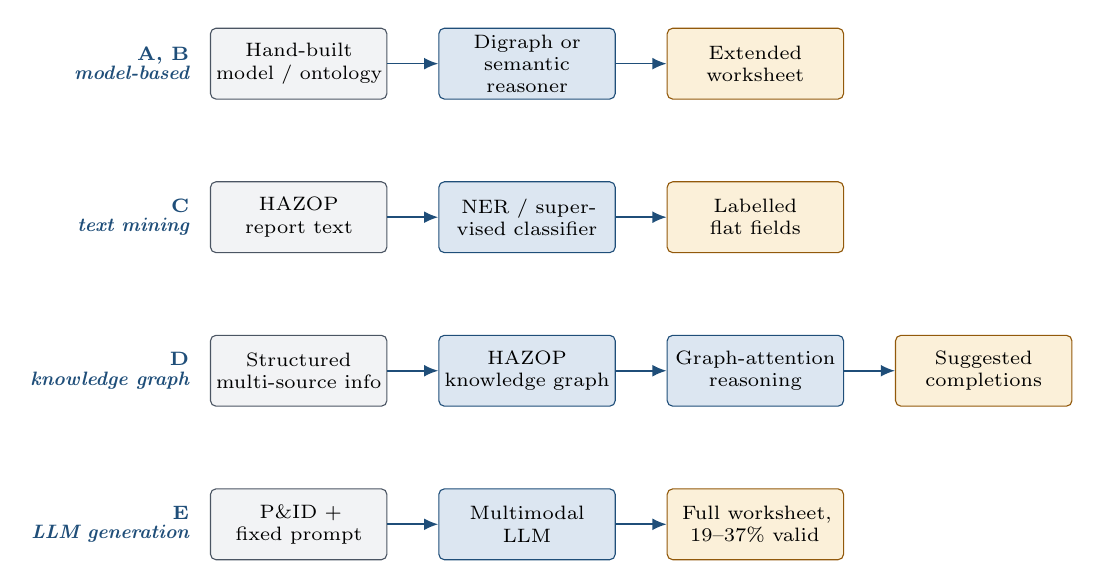
\begin{tikzpicture}[x=1cm,y=1cm]
  % column centres and row baselines
  \def\ca{0}   \def\cb{2.9} \def\cc{5.8} \def\cd{8.7}
  \def\ra{0}   \def\rb{-1.95} \def\rc{-3.9} \def\rd{-5.85}

  % --- lane A/B: hand-built model or ontology
  \node[lane,anchor=east] at (\ca-1.35,\ra) {A,~B\\[-1pt]\itshape model-based};
  \node[art,anchor=center]  (a1) at (\ca,\ra) {Hand-built model / ontology};
  \node[proc,anchor=center] (a2) at (\cb,\ra) {Digraph or semantic reasoner};
  \node[outc,anchor=center] (a3) at (\cc,\ra) {Extended worksheet};
  \draw[ar] (a1) -- (a2);  \draw[ar] (a2) -- (a3);

  % --- lane C: text mining, no graph
  \node[lane,anchor=east] at (\ca-1.35,\rb) {C\\[-1pt]\itshape text mining};
  \node[art,anchor=center]  (c1) at (\ca,\rb) {HAZOP report text};
  \node[proc,anchor=center] (c2) at (\cb,\rb) {NER / supervised classifier};
  \node[outc,anchor=center] (c3) at (\cc,\rb) {Labelled flat fields};
  \draw[ar] (c1) -- (c2);  \draw[ar] (c2) -- (c3);

  % --- lane D: knowledge graph + learned reasoning
  \node[lane,anchor=east] at (\ca-1.35,\rc) {D\\[-1pt]\itshape knowledge graph};
  \node[art,anchor=center]  (d1) at (\ca,\rc) {Structured multi-source info};
  \node[proc,anchor=center] (d2) at (\cb,\rc) {HAZOP knowledge graph};
  \node[proc,anchor=center] (d3) at (\cc,\rc) {Graph-attention reasoning};
  \node[outc,anchor=center] (d4) at (\cd,\rc) {Suggested completions};
  \draw[ar] (d1) -- (d2);  \draw[ar] (d2) -- (d3);  \draw[ar] (d3) -- (d4);

  % --- lane E: unconstrained generation
  \node[lane,anchor=east] at (\ca-1.35,\rd) {E\\[-1pt]\itshape LLM generation};
  \node[art,anchor=center]  (e1) at (\ca,\rd) {P\&ID + fixed prompt};
  \node[proc,anchor=center] (e2) at (\cb,\rd) {Multimodal LLM};
  \node[outc,anchor=center] (e3) at (\cc,\rd) {Full worksheet, 19--37\% valid};
  \draw[ar] (e1) -- (e2);  \draw[ar] (e2) -- (e3);
\end{tikzpicture}
\caption[Where each literature family gets its structure from]{The five
categories differ less in whether they use a graph than in where the
structure comes from and what is done with it. Grey boxes are inputs, blue
boxes are processing steps, amber boxes are outputs. Only Category C starts
from report text, and it is the one family that never builds a graph.}
\label{fig:lanes}
\end{figure}

\section{Capability Analysis}
The most important comparison axis identified in this review is the distinction between five operations that are frequently conflated in this literature:
\begin{enumerate}
  \item \textbf{Extraction} --- does the method pull information out of text (entities, spans, labels)?
  \item \textbf{Representation} --- does it explicitly represent relationships (graph, ontology), or only flat fields?
  \item \textbf{Causal reasoning} --- does it operate over those relationships to derive new statements, or merely store them?
  \item \textbf{Inference} --- does it produce previously unstated information (a missing cause, consequence, or safeguard)?
  \item \textbf{Validation} --- is the inferred output checked against expert judgment, process knowledge, or another ground truth?
\end{enumerate}
A paper should not be classified as performing causal reasoning merely because its output table contains fields labeled ``cause'' and ``consequence.'' Applying this test across the five categories gives Table~\ref{tab:capability}.

\begin{table}[htbp]
\centering
\caption[Capability matrix across the five literature categories]{Capability
matrix. \yes~= performed, \prt~= partial or method-dependent, \no~= not
performed. \emph{Validation} records whether validation was attempted, not
whether it succeeded --- Category E validates carefully and reports a poor
result. The last row is the profile this project would have to occupy to be
distinct; it is a target, not a result.}
\label{tab:capability}
\small
\resizebox{\columnwidth}{!}{%
\begin{tabularx}{\textwidth}{@{}l>{\raggedright\arraybackslash}Xccccc@{}}
\toprule
\textbf{Cat.} & \textbf{Primary input} & \textbf{Extr.} & \textbf{Repr.} & \textbf{Causal reas.} & \textbf{Infer.} & \textbf{Valid.} \\
\midrule
A & Hand-built process model (digraph, D-higraph) & \no  & \yes & \yes & \yes & \prt \\
B & Manually authored ontology                    & \no  & \yes & \yes & \yes & \yes \\
C & HAZOP report text                             & \yes & \no  & \no  & \no  & \prt \\
D & Structured multi-source information + ontology & \prt & \yes & \yes & \yes & \yes \\
E & P\&ID + standardized prompt                   & n/a  & \no  & \prt & \yes & \yes \\
\midrule
\textbf{Target} & Unstructured historical report text     & \yes & \yes & \yes & \yes & \yes \\
\bottomrule
\end{tabularx}
}%
\end{table}

Under this test, the Category C papers (Ekramipooya et al.\ 2023, 2024; Wang \& Gu 2022) perform extraction and classification but not causal reasoning: for example, Ekramipooya et al.\ (2023) predicts a deviation \emph{category} from cause text via supervised classification on a small dataset (three process nodes, 25 records, 42 after oversampling), which is correlational pattern-matching rather than reasoning over a causal structure.

\section{Important Findings}

\subsection{Single et al.\ (2020)}
This paper already provides ontology-based automated HAZOP reasoning. It models semantic/causal relationships between HAZOP concepts and uses a semantic reasoner to generate extended HAZOP worksheets, explicitly addressing the risk of automatically generated but meaningless scenarios through semantic constraints. Validation was performed on a hexane storage tank case study, where the quality and quantity of the automatically generated results agreed with the original expert worksheets.

\begin{constraint}[Constraint on the write-up]
The report must not claim that existing work fails to perform causal HAZOP
reasoning. Single et al.\ (2020) already does, and validates it against
expert worksheets.
\end{constraint}

Open questions requiring deeper reading: What exactly is the input (free text vs.\ pre-encoded knowledge)? How much of the ontology is manually authored per new process? How are causal chains represented internally? What precisely does the inference mechanism infer, and how dependent is it on predefined process knowledge?

\subsection{HAZOPCT --- Li \& Zhao (2025)}
This paper is closer still to the initially proposed direction. It constructs a HAZOP knowledge graph from multi-source process-safety information organized under a predefined ontology, then applies graph-attention-based reasoning over that graph to generate recommended conclusions for completing HAZOP analysis --- i.e., it performs missing-link inference, not just storage. It is evaluated on a sulfur-recovery-process case study, with ablation studies validating the contribution of semantic information and the graph-attention mechanism, and attention weights used to provide interpretability of the reasoning process.

\begin{constraint}[Constraint on the write-up]
The report must not claim that knowledge-graph-based HAZOP inference is
unexplored. HAZOPCT performs exactly this, with ablations and an
interpretability story.
\end{constraint}

Open questions requiring deeper reading: What is the raw input, and how much of the graph is manually curated versus text-extracted? What exactly are the node and edge types? What does ``completeness'' mean operationally in this paper? Does it reconstruct causal chains directly from unstructured HAZOP report text, or from already-structured data? Does it explicitly model intermediate causal events, or only direct cause--consequence links?

\section{Revision of Initial Assumptions}
The initial framing --- ``existing work only extracts HAZOP information, while this project introduces causal reasoning'' --- is not supportable given the findings above and has been discarded. The literature survey instead narrows the research problem before system design and evaluation.

\section{Provisional Research Direction}
One possible direction that survives the literature review, stated here only as a hypothesis, is reconstructing causal chains from \emph{unstructured, historical} HAZOP report text (as opposed to pre-encoded ontological knowledge) using LLM-based extraction, with the resulting chains constrained or validated against a structured graph rather than accepted at face value. Figure~\ref{fig:direction} sketches the shape of this pipeline and marks the two points where it would differ from existing work.

\begin{figure}[htbp]
\centering
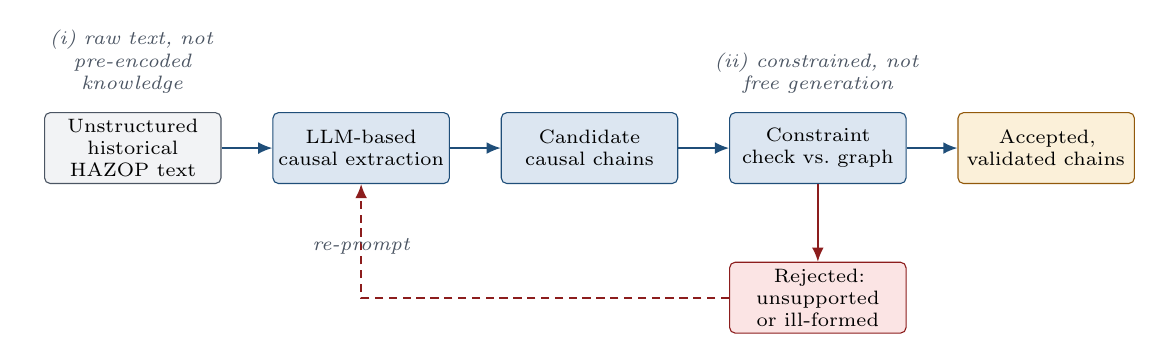
\begin{tikzpicture}[x=1cm,y=1cm]
  \node[art,anchor=center]  (p1) at (0,0)   {Unstructured historical HAZOP text};
  \node[proc,anchor=center] (p2) at (2.9,0) {LLM-based causal extraction};
  \node[proc,anchor=center] (p3) at (5.8,0) {Candidate causal chains};
  \node[proc,anchor=center] (p4) at (8.7,0) {Constraint check vs.\ graph};
  \node[outc,anchor=center] (p5) at (11.6,0) {Accepted, validated chains};
  \foreach \a/\b in {p1/p2,p2/p3,p3/p4,p4/p5} \draw[ar] (\a) -- (\b);

  % rejection path
  \node[art,anchor=center,draw=hzred,fill=hzredbg] (rej) at (8.7,-1.9)
        {Rejected: unsupported or ill-formed};
  \draw[ar,hzred] (p4) -- (rej);
  \draw[ar,hzred,densely dashed] (rej) -| (2.9,-1.9) -- (p2)
        node[tag,pos=0.62,below=1mm] {re-prompt};

  % the two claimed differences
  \node[tag,above=2mm of p1,text width=26mm] {(i) raw text, not\\ pre-encoded knowledge};
  \node[tag,above=2mm of p4,text width=26mm] {(ii) constrained, not\\ free generation};
\end{tikzpicture}
\caption[Provisional research direction]{Provisional pipeline. The two
annotations are the only points at which it currently claims to differ from
existing work, and both depend on readings that have not yet been done:
(i) assumes Single et al.\ and HAZOPCT work from pre-structured knowledge,
and (ii) responds to the low scenario validity of unconstrained LLM output.}
\label{fig:direction}
\end{figure}

This is motivated by two observations that still require confirmation: (i) Single et al.\ and HAZOPCT appear to reason over knowledge that is substantially pre-structured rather than reconstructed from raw report text; (ii) Lee et al.\ (2026) \cite{lee2026llmhazop} found that unconstrained LLM generation of full HAZOP worksheets achieved high textual similarity to expert references but only 19--37\% scenario validity, with safeguards skewed toward procedural rather than design-level interventions, suggesting raw LLM output is not reliable without some form of structural constraint.

\begin{provisional}[Status of this direction]
This is not yet a defensible novelty claim and must not be presented as the
final research gap until Single et al.\ (2020) and HAZOPCT have been read in
full. Both premises (i) and (ii) above are assumptions about papers not yet
read closely.
\end{provisional}

\section{Open Questions}
\begin{itemize}
  \item Does Single et al.\ (2020) operate on free text at all, or exclusively on pre-encoded ontological knowledge?
  \item What is the actual node/edge schema in HAZOPCT, and does it model intermediate causal events or only direct links?
  \item Is ``completeness'' in HAZOPCT defined relative to a fixed schema of expected fields, or relative to open-ended causal chain reconstruction?
  \item How much manual encoding effort does each approach require per new process, and does this scale to arbitrary historical report corpora?
  \item Does either paper attempt cross-report generalization, or are results confined to a single case-study process?
\end{itemize}

\section{Directions for Further Research}
\begin{enumerate}
  \item Full read of Single et al.\ (2020), answering the open questions listed above.
  \item Full read of Li \& Zhao (2025, HAZOPCT), answering the open questions listed above.
  \item Re-evaluate the provisional research direction in light of these two full reads.
  \item Only after this: attempt a first defensible statement of the research gap.
\end{enumerate}

% ------------------------------------------------------------
% NOTE: Bibliography
% See references.bib for BibTeX entries. Entries marked
% "% VERIFY" have incomplete or unconfirmed venue/DOI/page
% information pulled from secondary citations rather than the
% primary source, and must be checked before this log is
% finalized. No DOI has been invented; unverified DOIs are
% left blank rather than guessed.
% ------------------------------------------------------------

% ============================================================
% Week 02 section --- NLP for Structured HAZOP Reasoning
%
% Full read of Single et al. (2020), completed this week:
% architecture, ontology, inference engine, causal reasoning
% representation, the hexane storage-tank case study, results,
% comparison against the expert HAZOP, limitations, and future
% work. HAZOPCT (Li & Zhao, 2025) has not been started and
% carries forward to Week 03.
% ============================================================

\chapter[Ontology-Based HAZOP Reasoning]{Ontology-Based HAZOP Reasoning: A Detailed Analysis}

\section{Objective}
The objective was to understand Single et al.\ (2020) in enough depth to state precisely what the system does, what it assumes, and what it does not attempt. The analysis distinguishes throughout between what the paper itself establishes and our interpretation of its relevance to this project.

\section{Paper Studied}
Single, J. I., Schmidt, J., and Denecke, J.\ (2020). ``Ontology-based computer aid for the automation of HAZOP studies.'' \emph{Journal of Loss Prevention in the Process Industries}, 68, 104321 \cite{single2020ontologyhazop}.

\section{Problem Addressed by Single et al.}
The paper addresses the automated \emph{generation} of HAZOP worksheets for a given process unit, using a formally represented ontology of HAZOP-relevant knowledge together with a symbolic inference engine. As established in the literature survey, this is a generation problem, not an extraction problem: the system is not given a historical HAZOP report and asked to recover its reasoning; it is given a process-unit model and an ontology of causal/safety knowledge, and asked to produce a HAZOP worksheet from scratch.

\section{System Architecture}
The system requires, as input, structured knowledge about a process unit and its context: the process unit itself, its equipment, the substance(s) involved and their relevant properties, the process, and the circumstances under which it operates. \textbf{This knowledge is already available to the inference system before reasoning begins} --- the system does not discover it from raw text. Figure~\ref{fig:w2-arch} summarizes the architecture at this level.

\begin{figure}[htbp]
\centering
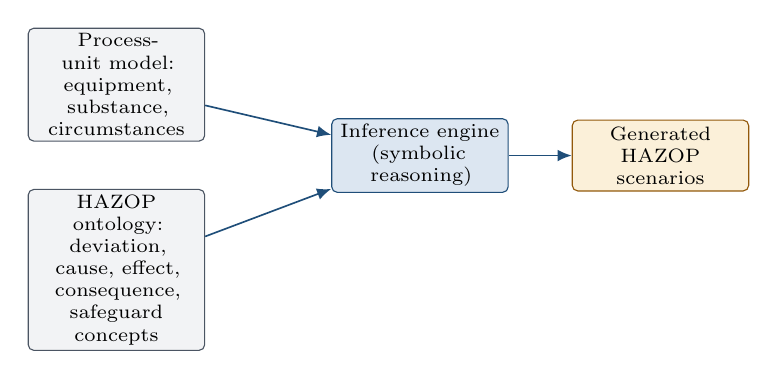
\begin{tikzpicture}[node distance=6mm and 8mm]
  \node[art] (pu) {Process-unit model: equipment, substance, circumstances};
  \node[art,below=of pu] (ont) {HAZOP ontology: deviation, cause, effect, consequence, safeguard concepts};
  \node[proc,right=16mm of pu,yshift=-9mm] (inf) {Inference engine (symbolic reasoning)};
  \node[outc,right=of inf] (out) {Generated HAZOP scenarios};
  \draw[ar] (pu) -- (inf);
  \draw[ar] (ont) -- (inf);
  \draw[ar] (inf) -- (out);
\end{tikzpicture}
\caption[System architecture of Single et al.\ (2020)]{The process-unit model and the HAZOP ontology are both supplied as structured input; the inference engine consumes both to produce scenarios. Neither the process-unit model nor the ontology is derived from unstructured report text in this system.}
\label{fig:w2-arch}
\end{figure}

\textbf{Our interpretation:} this places the entire knowledge-acquisition burden --- building the process-unit model and populating the ontology --- outside the automated part of the system. What is automated is the reasoning step, not the knowledge-entry step.

\section{HAZOP Ontology}
The ontology represents the concepts needed for HAZOP reasoning: Deviation, Cause, Effect, Super Cause, Consequence, Safeguard, Process Unit, Equipment, Substance, Process, and Circumstances. Critically, these concepts are not flat fields --- the ontology encodes a causal structure among them, and this structure supports branching and multiple causes, not only single linear chains. Figure~\ref{fig:w2-ontology-chain} shows the general shape of the causal structure the ontology supports.

\begin{figure}[htbp]
\centering
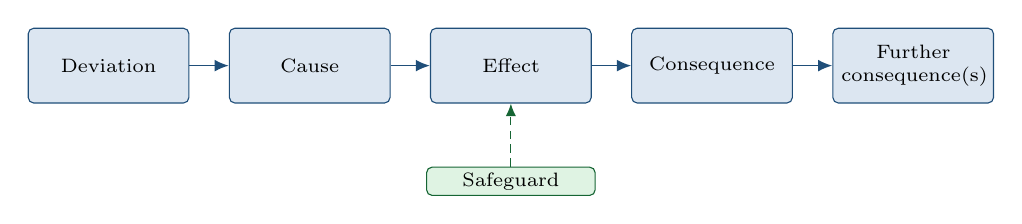
\begin{tikzpicture}[node distance=5mm and 5mm]
  \node[ev] (dev) {Deviation};
  \node[ev,right=of dev] (cause) {Cause};
  \node[ev,right=of cause] (eff) {Effect};
  \node[ev,right=of eff] (cons1) {Consequence};
  \node[ev,right=of cons1] (cons2) {Further consequence(s)};
  \node[sg,below=8mm of eff] (sgnode) {Safeguard};
  \draw[ar] (dev) -- (cause);
  \draw[ar] (cause) -- (eff);
  \draw[ar] (eff) -- (cons1);
  \draw[ar] (cons1) -- (cons2);
  \draw[sgar] (sgnode) -- (eff);
\end{tikzpicture}
\caption[General causal structure represented in the ontology]{The ontology's general causal structure. This is a template for the concepts and their ordering; the actual case-study instantiations (Section~\ref{sec:w2-casestudy}) show branching and multiple-cause variants of this same structure.}
\label{fig:w2-ontology-chain}
\end{figure}

Because the ontology encodes this structure explicitly rather than as flat worksheet fields, it is closer to a structured causal representation than to a conventional HAZOP table --- sharpening the observation that a flat worksheet is a presentational simplification of an underlying graph.

\section{Inference Engine}
The system's reasoning is implemented in OWL 2 DL, executed with the HermiT reasoner via Owlready2 in Python. \textbf{FACT:} this is symbolic, ontology-based reasoning, not statistical machine learning and not an LLM. The inference sequence described in the paper proceeds through five steps for a given deviation: identify causes, identify effects, identify super causes, identify consequences, and identify safeguards. The reasoner derives these by evaluating logical consequences of the modeled process information against the ontology's axioms, not by pattern-matching against text.

\section{Causal Reasoning Representation}
The paper's causal representation goes beyond simple one-to-one Deviation~$\rightarrow$~Cause or Cause~$\rightarrow$~Consequence links in three ways that are worth recording explicitly, since they matter for comparing this system against later knowledge-graph literature.

\paragraph{Multi-step chains.} A single deviation can propagate through several intermediate concepts before reaching a final consequence (Deviation~$\rightarrow$~Cause~$\rightarrow$~Effect~$\rightarrow$~Consequence~$\rightarrow$~further consequence(s)), matching the general structure in Figure~\ref{fig:w2-ontology-chain}.

\paragraph{Branching.} A single effect can lead to more than one distinct consequence path. Figure~\ref{fig:w2-branch} shows this using the loss-of-containment example from the case study (Section~\ref{sec:w2-casestudy}).

\begin{figure}[htbp]
\centering
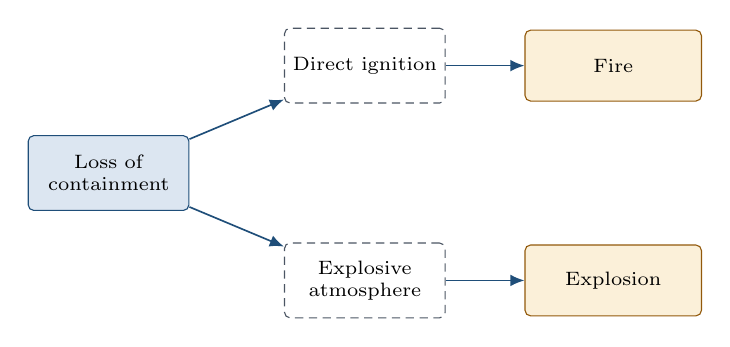
\begin{tikzpicture}[node distance=6mm and 10mm]
  \node[ev] (loc) {Loss of containment};
  \node[interev,above right=4mm and 12mm of loc] (ign) {Direct ignition};
  \node[interev,below right=4mm and 12mm of loc] (atm) {Explosive atmosphere};
  \node[outc,right=of ign] (fire) {Fire};
  \node[outc,right=of atm] (expl) {Explosion};
  \draw[ar] (loc) -- (ign);
  \draw[ar] (loc) -- (atm);
  \draw[ar] (ign) -- (fire);
  \draw[ar] (atm) -- (expl);
\end{tikzpicture}
\caption[Branching consequence paths]{A single effect (loss of containment) branching into two distinct consequence paths, as represented in the ontology.}
\label{fig:w2-branch}
\end{figure}

\paragraph{Multiple causes.} The ontology also supports several distinct causes converging on a single effect, rather than assuming each effect has exactly one cause.

\begin{figure}[htbp]
\centering
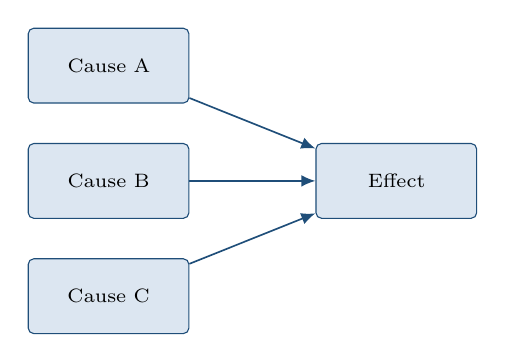
\begin{tikzpicture}[node distance=5mm and 8mm]
  \node[ev] (ca) {Cause A};
  \node[ev,below=of ca] (cb) {Cause B};
  \node[ev,below=of cb] (cc) {Cause C};
  \node[ev,right=16mm of cb] (eff) {Effect};
  \draw[ar] (ca) -- (eff);
  \draw[ar] (cb) -- (eff);
  \draw[ar] (cc) -- (eff);
\end{tikzpicture}
\caption[Multiple causes converging on one effect]{Multiple, independently modeled causes converging on a single effect.}
\label{fig:w2-multicause}
\end{figure}

\textbf{Our interpretation:} this branching/multi-cause capability is a genuine capability of the ontology's structure, not merely of the reasoning algorithm; it means the representation itself, not just the inference procedure, departs from a flat worksheet.

\section{Hexane Storage Tank Case Study}
\label{sec:w2-casestudy}
The methodology is demonstrated on a hexane storage tank. The process-unit model includes equipment such as valves, drain lines, a level control system, and a transfer/recirculation pump, together with hexane's safety-relevant properties. The original, human-authored HAZOP for this tank considers eight deviations: high level, low level, high temperature, low temperature, high pressure, low pressure, high concentration of contaminants, and loss of containment. The automated system generated 40 potential scenarios across these eight deviations.

One representative generated causal chain, given in the paper for the high-level deviation, is:

\begin{center}
\resizebox{\columnwidth}{!}{%
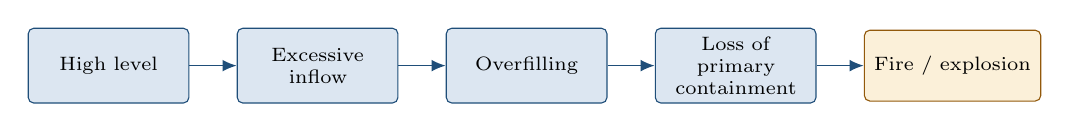
\begin{tikzpicture}[node distance=5mm and 6mm]
  \node[ev] (hl) {High level};
  \node[ev,right=of hl] (ei) {Excessive inflow};
  \node[ev,right=of ei] (of) {Overfilling};
  \node[ev,right=of of] (lopc) {Loss of primary containment};
  \node[outc,right=of lopc] (fe) {Fire / explosion};
  \foreach \a/\b in {hl/ei,ei/of,of/lopc,lopc/fe} \draw[ar] (\a) -- (\b);
\end{tikzpicture}
}%
\end{center}

The generated worksheet is structured with more fields than a conventional flat HAZOP table: Unit, Substance, Deviation, Super Cause, Cause, Effect, Consequence, and Safeguard, in place of the conventional Deviation / Cause / Consequence / Safeguard columns. Table~\ref{tab:w2-worksheet-fields} contrasts the two.

\begin{table}[htbp]
\centering
\caption[Conventional vs.\ generated worksheet fields]{Field structure of a conventional HAZOP worksheet compared with the fields in Single et al.'s generated worksheet. The additional fields (Unit, Substance, Super Cause, Effect) make intermediate causal steps explicit that the conventional table leaves implicit.}
\label{tab:w2-worksheet-fields}
\small
\begin{tabularx}{\columnwidth}{@{}>{\raggedright\arraybackslash}X>{\raggedright\arraybackslash}X@{}}
\toprule
\textbf{Conventional worksheet} & \textbf{Single et al.\ generated worksheet} \\
\midrule
Deviation & Unit \\
Cause & Substance \\
Consequence & Deviation \\
Safeguard & Super Cause \\
 & Cause \\
 & Effect \\
 & Consequence \\
 & Safeguard \\
\bottomrule
\end{tabularx}
\end{table}

\section{Automated HAZOP Results}
Beyond the field structure itself, the case study illustrates two representational points worth recording precisely.

\paragraph{Branching example.} The loss-of-containment scenario shown in Figure~\ref{fig:w2-branch} (direct ignition~$\rightarrow$~fire; explosive atmosphere~$\rightarrow$~explosion) is drawn directly from the case study's generated results, not a constructed illustration.

\paragraph{Guideword overlap.} The paper also discusses scenarios spanning more than one nominal deviation. A freezing-related scenario combines low temperature and water contamination as joint conditions:

\begin{center}
\resizebox{\columnwidth}{!}{%
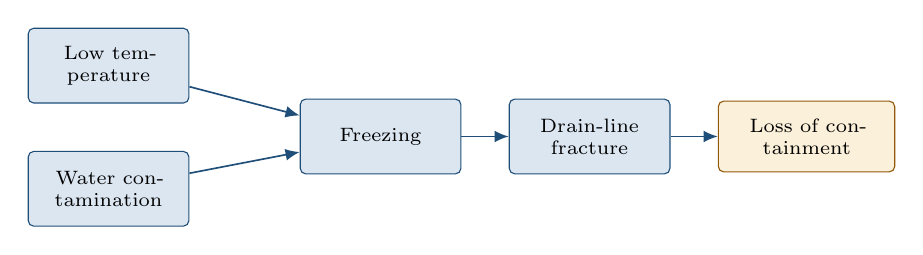
\begin{tikzpicture}[node distance=5mm and 6mm]
  \node[ev] (lt) {Low temperature};
  \node[ev,below=6mm of lt] (wc) {Water contamination};
  \node[ev,right=14mm of lt,yshift=-9mm] (fz) {Freezing};
  \node[ev,right=of fz] (df) {Drain-line fracture};
  \node[outc,right=of df] (loc2) {Loss of containment};
  \draw[ar] (lt) -- (fz);
  \draw[ar] (wc) -- (fz);
  \draw[ar] (fz) -- (df);
  \draw[ar] (df) -- (loc2);
\end{tikzpicture}
}%
\end{center}

\textbf{Our interpretation:} this shows a physical scenario does not always correspond cleanly to one deviation; a representation limited to ``one deviation $\rightarrow$ one scenario'' would not capture this case. Whether a future representation needs to support multiple joint conditions leading to one physical event is a design question raised by this example, not one the paper itself sets out to solve.

\section{Comparison with Expert HAZOP}
The paper compares the automatically generated results against the original expert HAZOP for the same tank. Table~\ref{tab:w2-comparison} reports the counts given in the paper.

\begin{table}[htbp]
\centering
\caption[Causes and consequences: original vs.\ automated]{Counts of causes and consequences in the original expert HAZOP versus the automatically generated worksheet, as reported by Single et al.}
\label{tab:w2-comparison}
\begin{tabular}{@{}lcc@{}}
\toprule
 & \textbf{Original (expert)} & \textbf{Automated} \\
\midrule
Causes        & 22 & 33 \\
Consequences  & 13 & 28 \\
\bottomrule
\end{tabular}
\end{table}

\begin{constraint}[Constraint on interpreting this comparison]
A larger count of generated causes and consequences must not be read as
evidence that the automated system is more correct or more complete than
the expert HAZOP. The paper itself emphasizes the continued need for
expert qualitative assessment of the generated results; quantity is not a
validity metric.
\end{constraint}

A further observation from the comparison is terminological rather than structural: the automated system and the human-authored HAZOP sometimes describe the same underlying physical situation using different terminology or a different level of abstraction. \textbf{Our interpretation:} this is directly relevant to any future text-extraction approach, since a system reading historical HAZOP report text would need to handle synonyms, varying abstraction levels, implicit causal relationships, and differing expert writing styles --- the problem is not reducible to matching exact phrases, even in a setting (like this one) where the comparison is between two already-structured outputs rather than between structured output and free text.

\section{Key Observations}
The paper distinguishes conceptually between preventive and mitigative safeguards, and notes that safeguards can attach to different points along a causal chain rather than to the scenario as a whole (consistent with the causal-chain representation illustrated earlier in this paper). However, the authors are explicit that safeguard and recommendation selection depends heavily on company practices, regulations, technical standards, industry context, and risk assessment --- meaning generated safeguards still require human expert evaluation before use. The overall workflow is therefore human-in-the-loop, not autonomous end to end: ontology $\rightarrow$ automated inference $\rightarrow$ generated scenarios $\rightarrow$ human expert evaluation $\rightarrow$ final assessment, with experts still needed for plausibility, likelihood, severity, safeguard adequacy, and recommendations.

\section{Limitations and Dependencies}
The following limitations and dependencies are identified from the paper; they are not exaggerated beyond what the source supports.

\begin{enumerate}
  \item Causal knowledge is encoded into the ontology beforehand, not discovered at run time.
  \item Result completeness depends directly on ontology completeness.
  \item The demonstrated case is equipment- / process-unit-level, not plant-wide.
  \item Plant-wide interactions between units are not fully addressed.
  \item Process-unit and P\&ID information is not automatically extracted in the demonstrated system --- it is modeled manually.
  \item Human expert validation of generated scenarios remains necessary.
  \item Risk assessment (likelihood, severity) is not fully automated.
  \item Safeguard selection remains context-dependent on company/regulatory practice.
  \item New or unrepresented causal knowledge requires ontology extension by a knowledge engineer.
  \item The demonstrated system is not a free-text HAZOP report understanding system.
\end{enumerate}

The central dependency underlying most of the above can be summarized as a knowledge-acquisition bottleneck (Figure~\ref{fig:w2-bottleneck}): the inference step is automated, but the acquisition and encoding of causal knowledge into the ontology is not.

\begin{figure}[htbp]
\centering
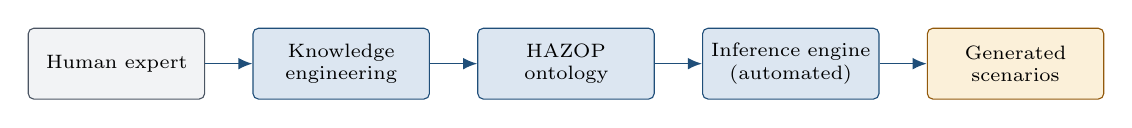
\begin{tikzpicture}[node distance=6mm and 6mm]
  \node[art] (he) {Human expert};
  \node[proc,right=of he] (ke) {Knowledge engineering};
  \node[proc,right=of ke] (ont) {HAZOP ontology};
  \node[proc,right=of ont] (inf) {Inference engine (automated)};
  \node[outc,right=of inf] (out) {Generated scenarios};
  \foreach \a/\b in {he/ke,ke/ont,ont/inf,inf/out} \draw[ar] (\a) -- (\b);
\end{tikzpicture}
\caption[Knowledge-acquisition bottleneck]{Only the inference step (fourth box) is automated; the preceding knowledge-engineering step remains a manual, expert-driven dependency.}
\label{fig:w2-bottleneck}
\end{figure}

The paper's stated future work includes: integration with broader industrial/process ontologies, integration with ISO~15926, integration with OntoCAPE, incorporating safety and security considerations, a sharper distinction between safeguards and recommendations, extraction of process-unit/equipment information from intelligent P\&IDs, and propagation of deviations/effects through upstream and downstream process nodes. \textbf{Our interpretation:} the ``extraction of process-unit/equipment information from intelligent P\&IDs'' item is the closest the paper comes to acknowledging its own knowledge-acquisition bottleneck as future work, though it is framed around P\&ID data rather than historical report text.

\section{Relevance to Our Research}
\begin{provisional}[How this paper relates to our provisional direction --- not a finalized gap]
Single et al.\ demonstrate: structured HAZOP knowledge + a process-unit model
+ symbolic inference $\rightarrow$ multi-step HAZOP causal scenarios, including
branching and multiple-cause chains. They do \emph{not} demonstrate: raw
HAZOP report text $\rightarrow$ automatic causal knowledge extraction
$\rightarrow$ causal graph $\rightarrow$ reasoning. This distinction, first
raised in the initial research framing, is now grounded in a full read of the
paper rather than an abstract-level reading. It provides a reference
architecture for the \emph{reasoning} half of a possible pipeline --- what
structured causal representation and symbolic reasoning over it can look
like --- but says nothing about whether the \emph{knowledge-acquisition}
half (currently manual, per Section~\ref{sec:w2-casestudy} and the
limitations above) could be replaced by text-based extraction. This
remains a research question, not a research gap: HAZOPCT and the
Category~C/D papers have not yet been read at this depth, and
any one of them could already address this question in ways this paper
does not.
\end{provisional}

\section{Relevance of Single et al. to Our Research Direction}
The detailed analysis above clarifies what Single et al.\ contributes to our
project and, equally importantly, what remains outside its scope. Our current
working hypothesis is not simply to extract entities from HAZOP reports. Given
historical HAZOP reports, we want to investigate whether a system can recover
the causal reasoning embedded in those reports and represent it in a form that
a machine can subsequently reason over. The conceptual pipeline is:

\begin{figure}[htbp]
\centering
\resizebox{\linewidth}{!}{%

\begin{tikzpicture}[node distance=4mm]
  \node[art] (r1) {Historical HAZOP reports};
  \node[proc,right=of r1] (r2) {NLP / LLM};
  \node[proc,right=of r2] (r3) {Causal information extraction};
  \node[proc,right=of r3] (r4) {Structured HAZOP knowledge};
  \node[proc,right=of r4] (r5) {Causal graph / ontology};
  \node[outc,right=of r5] (r6) {Reasoning / validation};
  \foreach \a/\b in {r1/r2,r2/r3,r3/r4,r4/r5,r5/r6}
    \draw[ar] (\a) -- (\b);
\end{tikzpicture}
}%
\caption[Current working pipeline for the project]{Conceptual pipeline
currently guiding the project. The pipeline is a working hypothesis rather
than a finalized system architecture or research gap.}
\label{fig:w2-our-pipeline}
\end{figure}

This direction distinguishes information extraction from causal reasoning.
Identifying a deviation, cause, consequence, and safeguard as isolated spans
does not establish how those concepts are related. For example, a report may
describe the chain
\emph{cooling-water failure} $\rightarrow$ \emph{temperature increase}
$\rightarrow$ \emph{pressure increase} $\rightarrow$ \emph{relief valve
opens}. A basic NLP system may detect each concept correctly while losing the
ordering, direction, intermediate events, or safeguard attachment. Our
research interest is therefore in reconstructing the causal chain itself:
information extraction is necessary, but information extraction is not causal
reasoning.

\begin{figure}[htbp]
\centering
\resizebox{\linewidth}{!}{%
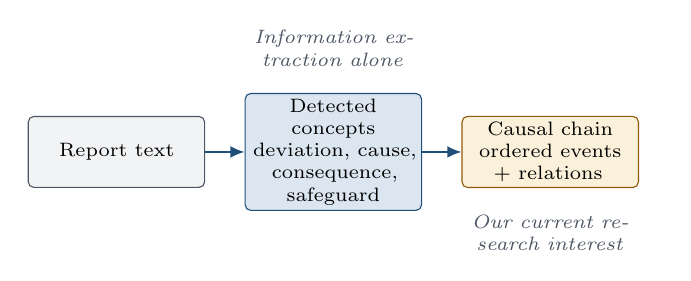
\begin{tikzpicture}[node distance=5mm]
  \node[art] (ie1) {Report text};
  \node[proc,right=of ie1] (ie2) {Detected concepts\\
    deviation, cause, consequence, safeguard};
  \node[outc,right=of ie2] (ie3) {Causal chain\\
    ordered events + relations};
  \draw[ar] (ie1) -- (ie2);
  \draw[ar] (ie2) -- (ie3);
  \node[tag,above=3mm of ie2,text width=28mm] {Information extraction alone};
  \node[tag,below=3mm of ie3,text width=28mm] {Our current research interest};
\end{tikzpicture}
}%
\caption[Information extraction versus causal reasoning]{Detecting HAZOP
concepts is an intermediate step; the intended research direction also
requires recovery of the relations and ordering that form a causal chain.}
\label{fig:w2-extraction-vs-reasoning}
\end{figure}

\paragraph{Single et al. as a reasoning reference.}
Single et al.\ provides a useful reference for the structured-reasoning side
of this project. Its ontology represents concepts including Process Unit,
Equipment, Substance, Deviation, Cause, Effect, Super Cause, Consequence, and
Safeguard, and its symbolic inference mechanism operates over relationships
among those concepts. It consequently helps answer the question: \emph{what
could a machine-readable representation of HAZOP causal reasoning look like?}
The ontology and its inferred chains provide a potential reasoning destination
that an NLP/LLM pipeline may eventually need to recover from historical
reports. This does not imply that the ontology is already the appropriate
schema for our data; the literature study must determine which concepts and
relations are required.

\paragraph{Difference between the two architectures.}
Conceptually, the architecture studied by Single et al.\ is:

\begin{center}
\emph{Expert knowledge} $\rightarrow$ \emph{ontology / structured process
knowledge} $\rightarrow$ \emph{symbolic inference} $\rightarrow$
\emph{generated HAZOP scenarios}.
\end{center}

Our current direction instead begins with historical documents:

\begin{center}
\emph{Historical HAZOP reports} $\rightarrow$ \emph{NLP / LLM} $\rightarrow$
\emph{causal knowledge extraction} $\rightarrow$ \emph{structured causal
representation} $\rightarrow$ \emph{reasoning / validation}.
\end{center}

The important distinction is not that Single et al.\ fails to automate HAZOP
analysis. It automates symbolic inference and demonstrates multi-step causal
reasoning. Rather, its architecture primarily assumes that the relevant
process and causal knowledge has already been formally represented. Our
interest is in the earlier knowledge-recovery stage and in connecting that
stage to reliable causal reasoning.

\begin{figure}[htbp]
\centering
\resizebox{\linewidth}{!}{%
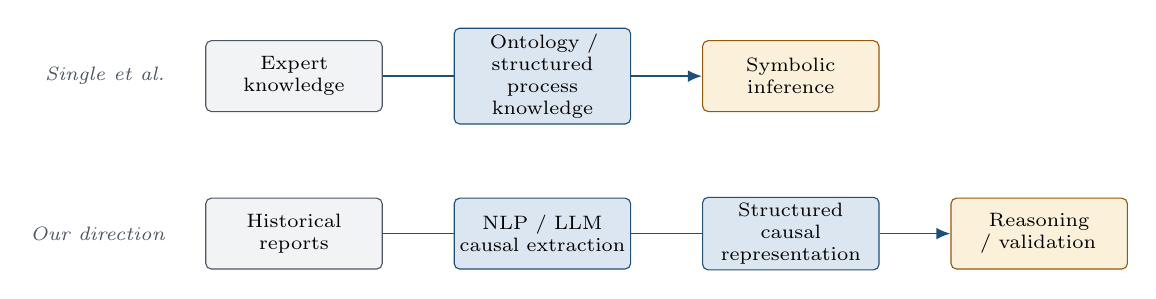
\begin{tikzpicture}[node distance=5mm and 9mm]
  \node[tag,anchor=east] at (-1.6,1.0) {Single et al.};
  \node[art] (s1) at (0,1.0) {Expert knowledge};
  \node[proc,right=of s1] (s2) {Ontology / structured\\process knowledge};
  \node[outc,right=of s2] (s3) {Symbolic inference};
  \draw[ar] (s1) -- (s2) -- (s3);

  \node[tag,anchor=east] at (-1.6,-1.0) {Our direction};
  \node[art] (o1) at (0,-1.0) {Historical reports};
  \node[proc,right=of o1] (o2) {NLP / LLM\\causal extraction};
  \node[proc,right=of o2] (o3) {Structured causal\\representation};
  \node[outc,right=of o3] (o4) {Reasoning / validation};
  \draw[ar] (o1) -- (o2) -- (o3) -- (o4);
\end{tikzpicture}
}%
\caption[Comparison of the two conceptual architectures]{Single et al.
assumes formally represented knowledge before inference, whereas our current
direction investigates the knowledge-recovery stages preceding reasoning.}
\label{fig:w2-architecture-comparison}
\end{figure}

This distinction also separates the present research direction from ordinary
document understanding or information-extraction work. Document understanding
asks what information can be found in a document. The HAZOP problem we are
formulating asks how the relationships and reasoning structure between pieces
of information can be recovered. The object of interest is therefore not only
the information present in the report, but the causal organization that makes
that information useful for safety analysis.

\paragraph{Potential uses of a recovered causal structure.}
If a structured causal graph could be constructed, it could potentially
support several future tasks. These are research questions, not capabilities
provided by the current system:

\begin{itemize}
  \item \textbf{Chain completeness:} given ``cooling failure $\rightarrow$
  temperature increases $\rightarrow$ ? $\rightarrow$ relief valve opens,''
  determine whether a missing intermediate event can be proposed or flagged.
  \item \textbf{Causal validity:} distinguish a plausible sequence from a
  questionable one, such as ``cooling failure $\rightarrow$ temperature
  decreases $\rightarrow$ pressure increases,'' using structured
  process-safety knowledge.
  \item \textbf{Semantic equivalence:} map statements such as ``cooling water
  failure causes reactor overheating'' and ``loss of coolant results in
  elevated reactor temperature'' to a common causal structure when their
  meanings are equivalent.
  \item \textbf{Missing-link inference:} propose relationships that are not
  explicitly recorded when historical reports contain only partial chains.
\end{itemize}

A possible representation is a graph in which nodes denote process-safety
concepts or events and edges denote relations such as \emph{causes},
\emph{leads to}, \emph{results in}, \emph{prevented by}, or \emph{mitigated
by}:

\begin{figure}[htbp]
\centering
\resizebox{\linewidth}{!}{%
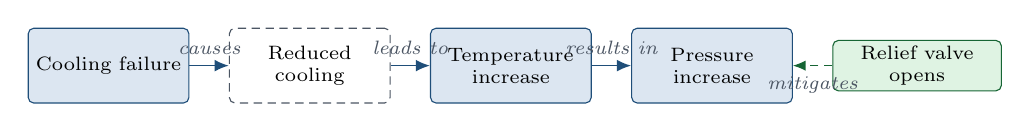
\begin{tikzpicture}[node distance=5mm]
  \node[ev] (g1) {Cooling failure};
  \node[interev,right=of g1] (g2) {Reduced cooling};
  \node[ev,right=of g2] (g3) {Temperature increase};
  \node[ev,right=of g3] (g4) {Pressure increase};
  \node[sg,right=of g4] (g5) {Relief valve opens};
  \draw[ar] (g1) -- node[tag,above=1mm] {causes} (g2);
  \draw[ar] (g2) -- node[tag,above=1mm] {leads to} (g3);
  \draw[ar] (g3) -- node[tag,above=1mm] {results in} (g4);
  \draw[sgar] (g5) -- node[tag,below=1mm] {mitigates} (g4);
\end{tikzpicture}
}%
\caption[Conceptual causal graph for HAZOP reasoning]{Illustrative causal
graph. Nodes represent process-safety events and edges represent possible
causal or safeguard relations; the schema is not yet finalized.}
\label{fig:w2-conceptual-graph}
\end{figure}

This is a conceptual example, not a finalized graph schema. A knowledge graph
could provide the intermediate representation between report-level language
and reasoning, but whether a knowledge graph, ontology, causal graph, or a
hybrid is most appropriate requires further investigation.

\paragraph{Open questions for our investigation.}
Single et al.\ does not by itself answer how causal relationships should be
extracted from raw HAZOP report text, how implicit causal relationships should
be detected, or how different expert terminology should be normalized. It
also leaves open how chains from multiple reports should be merged, how
previously unseen causal relationships should be handled, how LLM-generated
relationships should be validated, and how uncertainty in extracted
relationships should be represented. These are open questions that motivate
the subsequent literature analysis; they are not yet being presented as the
research gap.

The observations above define our current working research direction rather
than a finalized research gap. Subsequent papers, particularly later
knowledge-graph and HAZOP automation approaches, must be examined to determine
which parts of this pipeline have already been addressed.

\paragraph{Takeaway.}
Single et al.\ is useful to our project not because it directly solves our
intended problem, but because it provides an example of what structured HAZOP
causal reasoning can look like. It gives us a potential reasoning destination:
structured HAZOP knowledge $\rightarrow$ causal representation $\rightarrow$
symbolic reasoning. Our research is currently exploring how the earlier
stages can be connected: historical HAZOP reports $\rightarrow$ NLP/LLM
$\rightarrow$ causal structure $\rightarrow$ reasoning and validation. Later
literature will determine whether this distinction is genuinely novel.

\section{Questions for Subsequent Literature}
The following questions are added to the literature comparison framework and can be applied to HAZOPCT and other remaining papers:
\begin{enumerate}
  \item What is the input --- raw HAZOP report, P\&ID, structured process model, or ontology?
  \item Does the method perform information extraction (from text or from another unstructured source)?
  \item What representation is used --- flat table, ontology, knowledge graph, or causal graph?
  \item Does the method perform genuine causal reasoning, or only store labeled relationships?
  \item Does it support multi-hop causal chains, as Single et al.\ do?
  \item Does it infer missing causal relationships, or only reproduce encoded ones?
  \item How is reasoning validity evaluated, and against what?
  \item Is expert ground truth used for validation?
  \item How dependent is the method on predefined/manually encoded knowledge?
  \item Can it handle previously unseen causal relationships, or only combinations of known ones?
  \item Is the system equipment-level, process-unit-level, or plant-wide in scope?
\end{enumerate}

\section{Conclusions}
The full analysis of Single et al.\ (2020) shows that the paper performs genuine, multi-hop, branching causal reasoning over HAZOP concepts, evaluated against an expert worksheet on a real case study, and it does so entirely on the basis of manually encoded process and safety knowledge rather than on text extracted from historical reports. No research gap is being claimed on this basis. The open question for the project is whether the knowledge-acquisition step this system depends on --- and does not attempt to automate --- can be addressed by NLP/LLM-based extraction from historical report text, and whether the resulting extracted knowledge could be validated using reasoning structures similar to the one this paper demonstrates. HAZOPCT (Li \& Zhao, 2025) is the next knowledge-graph-based alternative to examine before this question is pursued further.

% ============================================================
% Week 03 section --- NLP for Structured HAZOP Reasoning
%
% Research planning and literature synthesis:
%   - Single et al. (2020)
%   - Mao et al. (2020)
%   - HAZOPCT / Li & Zhao (2025)
%   - Lee et al. (2026)
%
% This week moves from paper-by-paper analysis toward defining
% the case study, research questions, causal representation,
% experimental design, and validation strategy.
% ============================================================

\chapter[Literature Synthesis and Research Design]
{Literature Synthesis and Research Design}

\section{Objective}

The objective of this week was to consolidate the literature studied during
the previous weeks and use it to begin defining the research problem, case
study, and experimental methodology for the project. Rather than treating
the individual papers as isolated approaches, the analysis focuses on the
different stages involved in automated HAZOP analysis: knowledge
representation, information extraction, knowledge-graph construction,
causal reasoning, missing-relationship inference, and direct HAZOP
generation.

The purpose of this synthesis is not yet to claim a finalized research gap.
Instead, it is to determine which parts of the HAZOP reasoning pipeline have
already been addressed, what assumptions existing approaches make, and which
questions should be investigated through a focused case study.

\begin{glance}[Week 3 at a glance]
This week moves from reviewing individual automation approaches to defining
the project's research design. The central working direction is to extract
causal propositions from historical HAZOP reports, represent them explicitly,
and evaluate whether the resulting structure supports multi-hop reasoning.
The case study, schema, and ground-truth strategy remain provisional until
candidate datasets have been examined.
\end{glance}

\section{From Automated HAZOP Generation to Structured Causal Reasoning}

The literature studied so far suggests that ``automating HAZOP'' is not a
single technical problem. Different approaches automate different stages of
the overall process.

Single et al.\ (2020) demonstrate that HAZOP knowledge can be represented
using an ontology and that symbolic inference can be used to generate
multi-step HAZOP scenarios. Their system operates on an already structured
process and safety representation, with expert knowledge encoded in the
ontology before the reasoning process begins
\cite{single2020ontologyhazop}.

Mao et al.\ (2020) move the knowledge-acquisition problem closer to the
document level by developing a process-safety knowledge graph from
heterogeneous process-safety information. Their approach uses natural
language processing for named-entity recognition and relation extraction
from textual sources, including HAZOP reports. The resulting graph is then
used for applications including information retrieval and causal-chain
extraction \cite{mao2020processsafetykg}.

Li and Zhao's HAZOPCT (2025) extends the knowledge-graph direction toward
HAZOP completeness. Their approach constructs a HAZOP knowledge graph from
multiple sources and applies graph-based learning to predict potentially
missing relationships, allowing existing HAZOP information to be used for
the identification of additional conclusions
\cite{lizhao2025hazopct}.

Lee et al.\ (2026) investigate a different direction: direct generation of
complete HAZOP worksheets using multimodal large language models. Their
experiments show that LLM-generated worksheets can achieve high textual
similarity to expert-prepared worksheets, while the proportion of semantically
valid generated scenarios remains considerably lower. This distinction is
important because linguistic similarity alone does not establish the
correctness of a causal or process-safety argument
\cite{lee2026llmhazop}.

The four approaches therefore address different parts of the overall problem,
as summarized in Figure~\ref{fig:w3-literature-landscape}.

\begin{figure}[htbp]
\centering
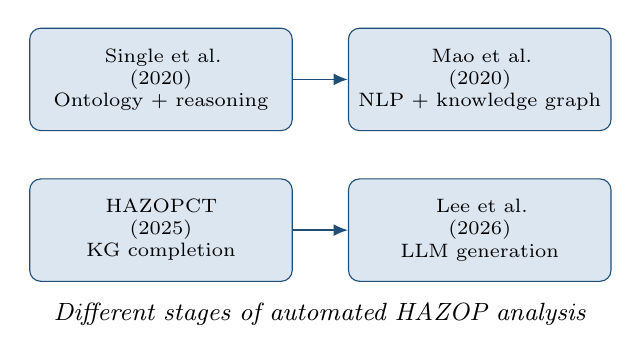
\begin{tikzpicture}[
    node distance=6mm and 7mm,
    box/.style={
        draw=hzblue,
        fill=hzbluebg,
        rounded corners,
        align=center,
        text width=31mm,
        minimum height=13mm,
        font=\scriptsize
    },
    arrow/.style={ar}
]

    \node[box] (single)
        {Single et al.\\(2020)\\
         Ontology + reasoning};

    \node[box, right=of single] (mao)
        {Mao et al.\\(2020)\\
         NLP + knowledge graph};

    \node[box, below=of single] (hazopct)
        {HAZOPCT\\(2025)\\
         KG completion};

    \node[box, right=of hazopct] (lee)
        {Lee et al.\\(2026)\\
         LLM generation};

    \node[below=8mm of $(hazopct)!0.5!(lee)$,
          align=center,
          text width=72mm,
          font=\small\itshape]
        (synthesis)
        {Different stages of automated HAZOP analysis};

    \draw[arrow] (single) -- (mao);
    \draw[arrow] (hazopct) -- (lee);

\end{tikzpicture}
\caption[Literature landscape for automated HAZOP analysis]
{The papers studied so far address different stages of automated HAZOP
analysis: structured symbolic reasoning, knowledge extraction and graph
construction, graph-based completion, and direct LLM-based generation.}
\label{fig:w3-literature-landscape}
\end{figure}

\section{A Layered View of the HAZOP Problem}

The comparison indicates that several capabilities must be distinguished when
discussing automated HAZOP analysis.

\begin{enumerate}
    \item \textbf{Information extraction:} identifying relevant entities,
    events, and relationships from documents.

    \item \textbf{Representation:} encoding extracted information using a
    structured representation such as a table, ontology, knowledge graph, or
    causal graph.

    \item \textbf{Causal reasoning:} determining how deviations, causes,
    effects, consequences, and safeguards are related and how events
    propagate through intermediate states.

    \item \textbf{Inference and validation:} identifying potentially missing
    relationships or scenarios and determining whether the resulting
    reasoning is consistent with process and safety knowledge.
\end{enumerate}

These capabilities are related but are not interchangeable. In particular,
identifying the concepts ``cooling failure'', ``high temperature'', and
``pressure increase'' does not by itself establish that they form an ordered
causal sequence.

The distinction is illustrated in Figure~\ref{fig:w3-layered-problem}.

\begin{figure}[htbp]
\centering
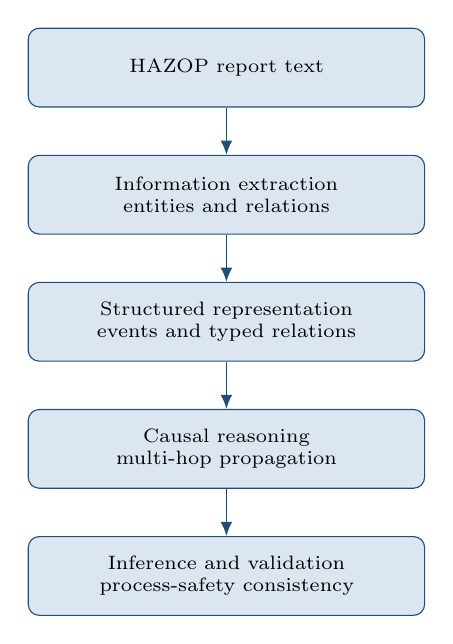
\begin{tikzpicture}[
    node distance=6mm,
    box/.style={
        draw=hzblue,
        fill=hzbluebg,
        rounded corners,
        align=center,
        text width=48mm,
        minimum height=10mm,
        font=\scriptsize
    },
    arrow/.style={ar}
]

    \node[box] (text)
        {HAZOP report text};

    \node[box, below=of text] (extract)
        {Information extraction\\
         entities and relations};

    \node[box, below=of extract] (repr)
        {Structured representation\\
         events and typed relations};

    \node[box, below=of repr] (reason)
        {Causal reasoning\\
         multi-hop propagation};

    \node[box, below=of reason] (valid)
        {Inference and validation\\
         process-safety consistency};

    \draw[arrow] (text) -- (extract);
    \draw[arrow] (extract) -- (repr);
    \draw[arrow] (repr) -- (reason);
    \draw[arrow] (reason) -- (valid);

\end{tikzpicture}
\caption[Layered view of automated HAZOP reasoning]
{A layered view of the HAZOP problem. Information extraction is an
intermediate step; causal reasoning additionally requires relationships,
direction, ordering, and propagation between events.}
\label{fig:w3-layered-problem}
\end{figure}

This distinction is particularly relevant to the present project. A system
may correctly identify individual HAZOP concepts while still failing to
recover the reasoning connecting those concepts.

\section{Why Causal Structure Is the Central Focus}

The literature studied so far suggests that the causal structure of HAZOP
information is more important than the presence of individual keywords alone.

Consider the following hypothetical description:

\begin{center}
\emph{Cooling-water failure may increase reactor temperature, which can cause
pressure buildup and ultimately result in loss of containment.}
\end{center}

A conventional information-extraction system may identify:

\begin{center}
\textit{cooling-water failure}, \quad
\textit{reactor temperature}, \quad
\textit{pressure buildup}, \quad
\textit{loss of containment}.
\end{center}

However, identifying these concepts does not establish the causal structure:

\begin{center}
\[
\text{Cooling failure}
\rightarrow
\text{Temperature increase}
\rightarrow
\text{Pressure increase}
\rightarrow
\text{Loss of containment}.
\]
\end{center}

The direction and ordering of these relationships are essential. A system
that detects all four concepts but assigns incorrect relationships has not
recovered the causal reasoning expressed by the original statement.

This distinction is also consistent with the progression of the literature.
Single et al.\ demonstrate that HAZOP reasoning can contain multi-step and
branching causal structures, while Mao et al.\ demonstrate how process-safety
information can be organized into a knowledge graph
\cite{single2020ontologyhazop,mao2020processsafetykg}.

The present investigation therefore focuses on the connection between
natural-language information and an explicit causal representation.

\section{Current Working Research Pipeline}

Based on the literature studied so far, the current working hypothesis is to
investigate a pipeline that begins with historical HAZOP reports rather than
with an already constructed process ontology.

The proposed high-level pipeline is:

\begin{center}
\emph{Historical HAZOP reports}
$\rightarrow$
\emph{NLP/LLM extraction}
$\rightarrow$
\emph{causal information}
$\rightarrow$
\emph{structured causal representation}
$\rightarrow$
\emph{causal reasoning}
$\rightarrow$
\emph{validation}.
\end{center}

Figure~\ref{fig:w3-working-pipeline} presents the same idea in a compact
system representation.

\begin{figure}[htbp]
\centering
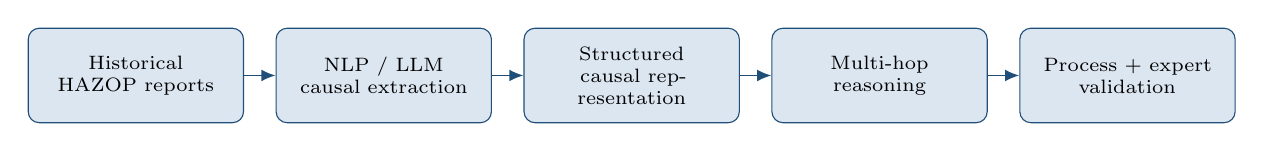
\begin{tikzpicture}[
    node distance=5mm and 4mm,
    box/.style={
        draw=hzblue,
        fill=hzbluebg,
        rounded corners,
        align=center,
        text width=25mm,
        minimum height=12mm,
        font=\scriptsize
    },
    arrow/.style={ar}
]

    \node[box] (reports)
        {Historical\\HAZOP reports};

    \node[box, right=of reports] (extract)
        {NLP / LLM\\
         causal extraction};

    \node[box, right=of extract] (graph)
        {Structured\\
         causal representation};

    \node[box, right=of graph] (reason)
        {Multi-hop\\
         reasoning};

    \node[box, right=of reason] (valid)
        {Process + expert\\
         validation};

    \draw[arrow] (reports) -- (extract);
    \draw[arrow] (extract) -- (graph);
    \draw[arrow] (graph) -- (reason);
    \draw[arrow] (reason) -- (valid);

\end{tikzpicture}
\caption[Current working research pipeline]
{Current working pipeline for investigating structured HAZOP reasoning from
historical reports. This is a working research hypothesis rather than a
finalized system architecture.}
\label{fig:w3-working-pipeline}
\end{figure}

The purpose of this pipeline is not to assume that a knowledge graph or a
particular ontology is already the correct representation. Instead, the
literature is being used to determine the representation and reasoning
requirements that the case study must satisfy.

In particular, the following questions remain open:

\begin{enumerate}
    \item Which HAZOP concepts need to be explicitly represented?

    \item Which relation types are required to distinguish causality from
    simple association?

    \item How should multi-step and branching causal chains be represented?

    \item How should multiple causes leading to a common effect be
    represented?

    \item How should safeguards be attached to causal chains?

    \item How should uncertainty in extracted relationships be represented?

    \item Can an extracted causal graph support reasoning over more than one
    causal hop?

    \item Can missing or incomplete causal relationships be identified?
\end{enumerate}

These questions will be used to define the case study and experimental
methodology in the subsequent sections of this week's report.

% ============================================================
% Week 03 --- Part II
% Case-study design and data requirements
% ============================================================

\section{Case-Study Design}

The literature review established that the central objective of this
research is not merely to identify HAZOP entities, but to recover the
causal structure connecting deviations, causes, consequences, and
safeguards. Therefore, the choice of case study is an important part of
the experimental design.

Rather than selecting a process solely because a HAZOP dataset is
available, the case study should provide sufficient causal structure
for evaluating information extraction and subsequent reasoning. The
selected process should also contain enough variation in terminology
and causal descriptions to test whether the proposed NLP/LLM approach
can generalize beyond a small collection of nearly identical sentences.

\subsection{Requirements for the Case Study}

The initial requirements for the case study are summarized in
Figure~\ref{fig:case-study-requirements}.

\begin{figure}[htbp]
\centering
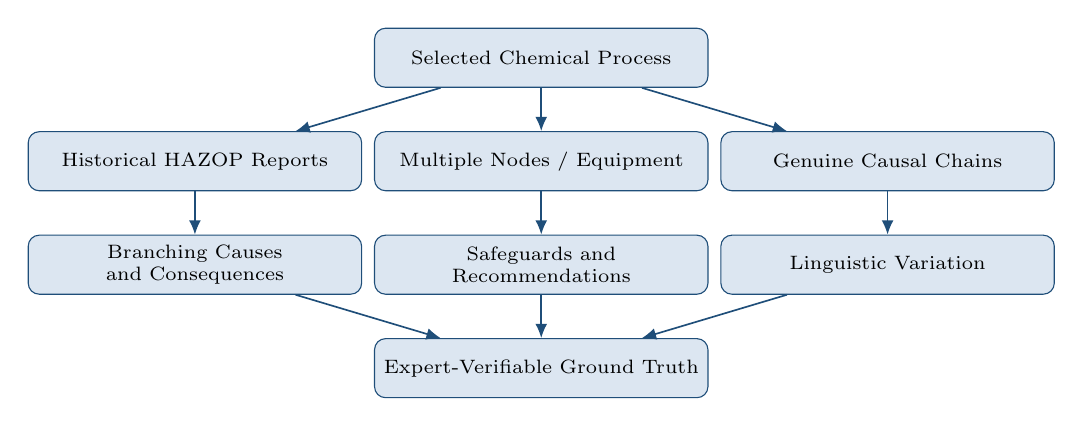
\begin{tikzpicture}[
    node distance=0.45cm,
    box/.style={
        rectangle,
        rounded corners,
        draw=hzblue,
        fill=hzbluebg,
        align=center,
        text width=4.0cm,
        minimum height=0.75cm,
        font=\scriptsize
    },
    arrow/.style={ar}
]

\node[box] (case) {Selected Chemical Process};

\node[box, below left=0.55cm and 0.15cm of case] (reports)
    {Historical HAZOP Reports};

\node[box, below=0.55cm of case] (nodes)
    {Multiple Nodes / Equipment};

\node[box, below right=0.55cm and 0.15cm of case] (chains)
    {Genuine Causal Chains};

\node[box, below=0.55cm of reports] (branch)
    {Branching Causes and Consequences};

\node[box, below=0.55cm of nodes] (safeguards)
    {Safeguards and Recommendations};

\node[box, below=0.55cm of chains] (variation)
    {Linguistic Variation};

\node[box, below=0.55cm of safeguards] (validation)
    {Expert-Verifiable Ground Truth};

\draw[arrow] (case) -- (reports);
\draw[arrow] (case) -- (nodes);
\draw[arrow] (case) -- (chains);

\draw[arrow] (reports) -- (branch);
\draw[arrow] (nodes) -- (safeguards);
\draw[arrow] (chains) -- (variation);

\draw[arrow] (branch) -- (validation);
\draw[arrow] (safeguards) -- (validation);
\draw[arrow] (variation) -- (validation);

\end{tikzpicture}
\caption{Initial requirements for selecting the case study.}
\label{fig:case-study-requirements}
\end{figure}

The following characteristics are considered desirable.

\begin{enumerate}[label=\textbf{\arabic*.}]

    \item \textbf{Availability of HAZOP reports:}
    The case study should have access to sufficiently detailed HAZOP
    worksheets or reports containing deviations, causes, consequences,
    safeguards, and relevant process context.

    \item \textbf{Multiple process nodes:}
    The process should contain multiple equipment items or HAZOP nodes
    so that the proposed method can be evaluated across different
    process contexts.

    \item \textbf{Explicit causal relationships:}
    The reports should contain statements from which causal
    relationships can be recovered rather than only isolated labels
    or keywords.

    \item \textbf{Multi-step causal chains:}
    The data should contain cases in which a cause produces an
    intermediate state or deviation that subsequently produces one or
    more consequences.

    \item \textbf{Branching structure:}
    Ideally, individual deviations should have multiple possible causes
    and consequences. This is important because a simple one-to-one
    mapping would not adequately test causal graph construction.

    \item \textbf{Safeguard information:}
    The HAZOP records should contain safeguards or recommendations so
    that the causal structure can eventually be connected to risk
    mitigation information.

    \item \textbf{Linguistic variation:}
    Different HAZOP entries should express similar causal relationships
    using different terminology or sentence structures. This allows
    the extraction system to be tested for semantic rather than
    purely lexical matching.

    \item \textbf{Expert-verifiable ground truth:}
    The extracted relationships and reconstructed causal chains should
    be capable of being checked against the original HAZOP analysis
    and, where possible, by a process-safety expert.

\end{enumerate}

\subsection{Why These Requirements Matter}

The requirements are motivated by the distinction between
information extraction and causal reasoning identified in the
literature.

For example, consider a simplified process-safety description:

\begin{center}
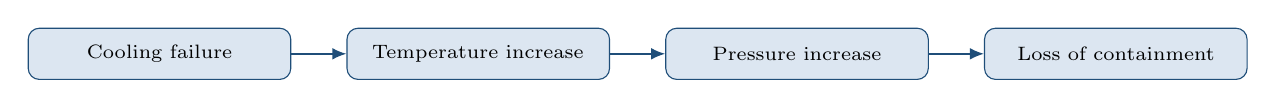
\begin{tikzpicture}[
    node distance=0.55cm,
    box/.style={
        rectangle,
        rounded corners,
        draw=hzblue,
        fill=hzbluebg,
        align=center,
        text width=3.1cm,
        minimum height=0.65cm,
        font=\scriptsize
    },
    arrow/.style={ar}
]

\node[box] (cause) {Cooling failure};
\node[box, right=0.7cm of cause] (temp) {Temperature increase};
\node[box, right=0.7cm of temp] (pressure) {Pressure increase};
\node[box, right=0.7cm of pressure] (loss) {Loss of containment};

\draw[arrow] (cause) -- (temp);
\draw[arrow] (temp) -- (pressure);
\draw[arrow] (pressure) -- (loss);

\end{tikzpicture}
\end{center}

In this example, identifying the four concepts is only the first
step. A useful system must also recover the relationships between
them. The resulting structure can be represented as

\begin{equation}
C_1 \rightarrow D_1 \rightarrow E_1 \rightarrow C_2,
\end{equation}

where the symbols represent successive causal states rather than
independent HAZOP entities.

Consequently, a case study containing only isolated statements such as
``high pressure'', ``valve failure'', or ``fire'' would be insufficient
for evaluating the main research objective. The dataset must contain
enough contextual information to determine how such concepts are
related.

\subsection{HAZOP Entry as the Basic Unit of Analysis}

The initial experimental unit will be an individual HAZOP entry or
worksheet row. A conventional entry can be viewed as containing
several semantically distinct components:

\begin{center}

\begin{tikzpicture}[
    node distance=0.45cm,
    box/.style={
        rectangle,
        rounded corners,
        draw=hzblue,
        fill=hzbluebg,
        align=center,
        text width=2.4cm,
        minimum height=0.65cm,
        font=\scriptsize
    },
    arrow/.style={ar}
]

\node[box] (node) {Node};
\node[box, right=0.35cm of node] (dev) {Deviation};
\node[box, right=0.35cm of dev] (cause) {Cause};
\node[box, right=0.35cm of cause] (effect) {Consequence};
\node[box, right=0.35cm of effect] (safe) {Safeguard};

\draw[arrow] (node) -- (dev);
\draw[arrow] (dev) -- (cause);
\draw[arrow] (cause) -- (effect);
\draw[arrow] (effect) -- (safe);

\end{tikzpicture}
\end{center}

This representation should not be interpreted as claiming that every
HAZOP entry forms a simple linear chain. Instead, it provides an
initial decomposition of the information contained in a worksheet.
The actual representation may contain multiple causes, intermediate
states, several consequences, and safeguards attached to different
parts of the causal structure.

\subsection{From HAZOP Rows to Causal Propositions}

A major objective of the case-study analysis will therefore be to
transform the textual information in a HAZOP entry into explicit
causal propositions.

For example, a textual entry could conceptually produce propositions
of the form

\begin{align}
\text{Cause} &\xrightarrow{\text{causes}} \text{Deviation},\\
\text{Deviation} &\xrightarrow{\text{leads\_to}} \text{Consequence},\\
\text{Consequence} &\xrightarrow{\text{mitigated\_by}} \text{Safeguard}.
\end{align}

The precise relation vocabulary is intentionally left open at this
stage. Determining whether these relations are sufficient, or whether
additional relations are required to represent intermediate process
states, is one of the questions to be investigated during the
subsequent design phase.

\subsection{Ground-Truth Construction}

The original HAZOP reports will serve as the primary source of
ground-truth information. However, the original worksheet structure
may not directly provide all of the intermediate causal links required
for evaluating multi-hop reasoning.

Therefore, the ground truth will be developed in stages:

\begin{enumerate}[label=\textbf{\arabic*.}]
    \item identify the relevant HAZOP entities in the source entry;
    \item identify explicitly stated causal relationships;
    \item identify multi-step relationships that are supported by the
    text and process context;
    \item represent alternative causes and consequences where they
    exist;
    \item associate safeguards with the corresponding causal scenario;
    \item obtain expert review for relationships that require process
    interpretation.
\end{enumerate}

This distinction is important because an automatically extracted graph
should not be treated as ground truth merely because the model
generated it. The reference structure must originate from the
available HAZOP evidence and, where necessary, expert assessment.

\subsection{Case-Study Selection Strategy}

At this stage, a specific process will not be selected solely on the
basis of convenience. Candidate datasets will instead be evaluated
against the requirements defined above.

The selection can be formulated as a screening process:

\begin{center}
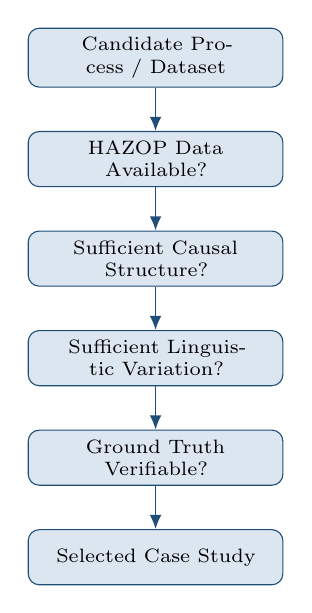
\begin{tikzpicture}[
    node distance=0.55cm,
    box/.style={
        rectangle,
        rounded corners,
        draw=hzblue,
        fill=hzbluebg,
        align=center,
        text width=3.0cm,
        minimum height=0.7cm,
        font=\scriptsize
    },
    arrow/.style={ar}
]

\node[box] (candidate) {Candidate Process / Dataset};

\node[box, below=0.55cm of candidate] (availability)
    {HAZOP Data Available?};

\node[box, below=0.55cm of availability] (structure)
    {Sufficient Causal Structure?};

\node[box, below=0.55cm of structure] (variation)
    {Sufficient Linguistic Variation?};

\node[box, below=0.55cm of variation] (validation)
    {Ground Truth Verifiable?};

\node[box, below=0.55cm of validation] (select)
    {Selected Case Study};

\draw[arrow] (candidate) -- (availability);
\draw[arrow] (availability) -- (structure);
\draw[arrow] (structure) -- (variation);
\draw[arrow] (variation) -- (validation);
\draw[arrow] (validation) -- (select);

\end{tikzpicture}
\end{center}

\subsection{Current Status}

The case-study process is therefore considered an open design
decision at this point. The immediate objective is to identify a
dataset that satisfies the causal and validation requirements rather
than to optimize for dataset size alone.

This approach also allows the research design to remain independent of
a particular process until the available HAZOP material has been
examined. Once candidate reports are obtained, their structure,
terminology, causal depth, branching, and available process context
can be compared against the requirements established in this section.

\subsection{Implications for the Experimental Design}

The case study will eventually support evaluation at several levels:

\begin{center}
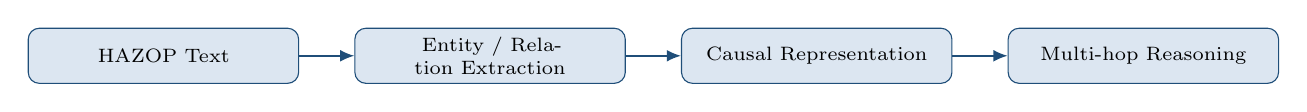
\begin{tikzpicture}[
    node distance=0.5cm,
    box/.style={
        rectangle,
        rounded corners,
        draw=hzblue,
        fill=hzbluebg,
        align=center,
        text width=3.2cm,
        minimum height=0.7cm,
        font=\scriptsize
    },
    arrow/.style={ar}
]

\node[box] (text) {HAZOP Text};
\node[box, right=0.7cm of text] (extract)
    {Entity / Relation Extraction};
\node[box, right=0.7cm of extract] (graph)
    {Causal Representation};
\node[box, right=0.7cm of graph] (reason)
    {Multi-hop Reasoning};

\draw[arrow] (text) -- (extract);
\draw[arrow] (extract) -- (graph);
\draw[arrow] (graph) -- (reason);

\end{tikzpicture}
\end{center}

This decomposition will make it possible to distinguish errors caused
by incorrect extraction from errors introduced during graph
construction or causal reasoning. Such separation is necessary for
determining whether an observed failure is an NLP problem, a
representation problem, or a reasoning problem.

The next stage of the research will therefore focus on examining
candidate HAZOP datasets and determining the exact causal schema that
can be reliably annotated from them.

% ============================================================
% Week 03 --- Part III
% Causal Schema, Experimental Design, and Next Steps
% ============================================================

\section{Causal Schema and Experimental Design}

The previous sections established the literature landscape and the
requirements for selecting a suitable HAZOP case study. The remaining
task is to define how the extracted information will be represented,
evaluated, and used for causal reasoning.

\subsection{Initial Causal Representation}

The working representation is based on typed entities and relationships
rather than the original tabular HAZOP format. The initial structure is:

\begin{center}
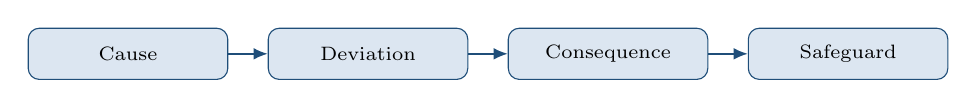
\begin{tikzpicture}[
    node distance=0.55cm,
    box/.style={
        rectangle,
        rounded corners,
        draw=hzblue,
        fill=hzbluebg,
        align=center,
        text width=2.3cm,
        minimum height=0.65cm,
        font=\scriptsize
    },
    arrow/.style={ar}
]

\node[box] (cause) {Cause};
\node[box, right=0.5cm of cause] (dev) {Deviation};
\node[box, right=0.5cm of dev] (cons) {Consequence};
\node[box, right=0.5cm of cons] (safe) {Safeguard};

\draw[arrow] (cause) -- (dev);
\draw[arrow] (dev) -- (cons);
\draw[arrow] (cons) -- (safe);

\end{tikzpicture}
\end{center}

This should not be interpreted as a restriction to linear chains. A
deviation may have multiple causes and consequences, while a
consequence may itself become an intermediate state in a longer causal
chain.

The representation can therefore be expressed as

\[
G=(V,E),
\]

where \(V\) contains entities and \(E\) contains typed relationships.

The initial entity types are:

\begin{center}
\begin{tabular}{ll}
\textbf{Entity} & \textbf{Description} \\
\hline
Process Node & HAZOP study location \\
Equipment & Physical equipment involved \\
Parameter & Process variable \\
Deviation & HAZOP deviation \\
Cause & Initiating or contributing condition \\
Consequence & Resulting outcome \\
Safeguard & Existing protective measure \\
Recommendation & Proposed protective action
\end{tabular}
\end{center}

The schema is provisional and will be revised after examination of the
selected HAZOP data.

\subsection{Causal Relations}

The initial relation vocabulary is:

\begin{center}
\begin{tabular}{ll}
\textbf{Relation} & \textbf{Meaning} \\
\hline
causes & Cause produces a deviation or state \\
leads\_to & One state produces another state or consequence \\
results\_in & Consequence relation \\
mitigated\_by & Protective measure associated with a scenario \\
associated\_with & Contextual association \\
has\_parameter & Equipment/node--parameter relationship \\
has\_deviation & Node--deviation relationship
\end{tabular}
\end{center}

The final relation vocabulary will be determined from the actual
language and causal structures present in the dataset.

\subsection{Annotation Strategy}

The basic annotation unit will be a causal proposition represented as

\[
(h,r,t),
\]

where \(h\) is the source entity, \(r\) is the relation, and \(t\) is
the target entity.

For example,

\[
(\text{Cooling Failure},\text{causes},\text{High Temperature})
\]

followed by

\[
(\text{High Temperature},\text{leads\_to},\text{Pressure Increase}).
\]

Multiple propositions can then be combined into a causal graph.

The annotation process will distinguish between:

\begin{enumerate}[label=\textbf{\arabic*.}]
    \item entities and process context;
    \item explicitly stated causal relationships;
    \item multi-step relationships;
    \item alternative causes and consequences;
    \item safeguards and recommendations.
\end{enumerate}

Implicit relationships that require substantial process interpretation
will be marked separately rather than automatically treated as
ground truth.

\subsection{Proposed Research Pipeline}

The complete working pipeline for the study is:

\begin{center}
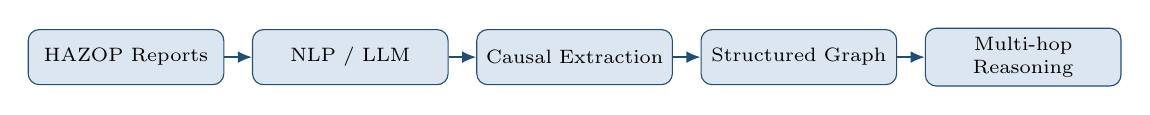
\begin{tikzpicture}[
    node distance=0.4cm,
    box/.style={
        rectangle,
        rounded corners,
        draw=hzblue,
        fill=hzbluebg,
        align=center,
        text width=2.25cm,
        minimum height=0.7cm,
        font=\scriptsize
    },
    arrow/.style={ar}
]

\node[box] (data) {HAZOP Reports};
\node[box, right=0.35cm of data] (extract) {NLP / LLM};
\node[box, right=0.35cm of extract] (causal) {Causal Extraction};
\node[box, right=0.35cm of causal] (graph) {Structured Graph};
\node[box, right=0.35cm of graph] (reason) {Multi-hop Reasoning};

\draw[arrow] (data) -- (extract);
\draw[arrow] (extract) -- (causal);
\draw[arrow] (causal) -- (graph);
\draw[arrow] (graph) -- (reason);

\end{tikzpicture}
\end{center}

The extracted structure will then be compared against the annotated
reference structure and evaluated for causal correctness.

\subsection{Experimental Comparison}

The initial experiments will compare different levels of extraction
and reasoning rather than evaluating only a single model.

\begin{description}[style=nextline,leftmargin=0pt,labelindent=0pt,font=\bfseries]

    \item[Experiment 1: Classical NLP baseline]

    A conventional pipeline using named entity recognition followed by
    relation extraction will provide a baseline for comparison.

    \item[Experiment 2: LLM structured extraction]

    An LLM will be prompted to extract HAZOP entities and typed causal
    relations into a predefined structured format.

    \item[Experiment 3: Explicit causal extraction]

    The extraction task will explicitly require identification of
    causal direction and intermediate states rather than simply
    identifying related entities.

    \item[Experiment 4: Causal graph reasoning]

    The extracted relations will be assembled into a graph and used
    for multi-hop reasoning.

    \item[Experiment 5: Missing-relation experiment]

    Known relationships can be temporarily removed from the graph and
    the system can be tested on whether it can recover the missing
    relationship or causal path.

\end{description}

The last experiment is particularly relevant to the distinction
between extraction and reasoning. A system that merely reproduces
information from the input is different from one that can use an
existing causal structure to identify a missing relationship.

\subsection{Evaluation Metrics}

Evaluation will be performed at multiple levels.

\begin{center}
\begin{tabular}{ll}
\textbf{Level} & \textbf{Possible Metrics} \\
\hline
Entity extraction & Precision, Recall, F1 \\
Relation extraction & Precision, Recall, F1 \\
Causal direction & Relation accuracy \\
Causal chains & Path Precision, Recall, F1 \\
Multi-hop reasoning & 1-hop / 2-hop / 3-hop accuracy \\
Missing relationships & Recovery accuracy, false positives \\
Safety validity & Expert/process-safety assessment
\end{tabular}
\end{center}

This separation is important because a system may achieve good entity
recognition while still producing incorrect causal relationships.

Similarly, correct relation extraction does not necessarily imply
successful multi-hop reasoning.

\subsection{Validation Strategy}

The final evaluation should therefore include both computational and
domain-based validation.

\begin{center}
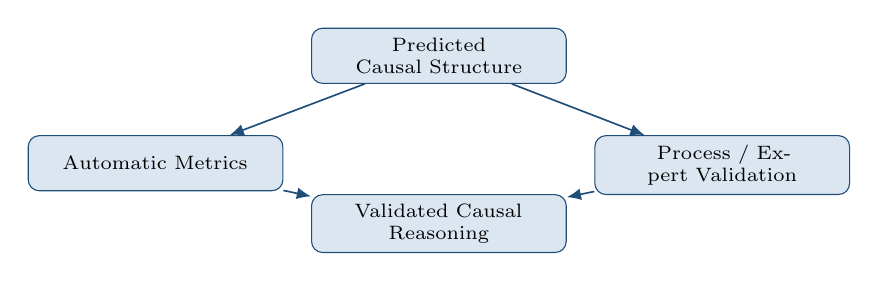
\begin{tikzpicture}[
    node distance=0.55cm,
    box/.style={
        rectangle,
        rounded corners,
        draw=hzblue,
        fill=hzbluebg,
        align=center,
        text width=3.0cm,
        minimum height=0.7cm,
        font=\scriptsize
    },
    arrow/.style={ar}
]

\node[box] (prediction) {Predicted Causal Structure};

\node[box, below left=0.65cm and 0.35cm of prediction]
    (metric) {Automatic Metrics};

\node[box, below right=0.65cm and 0.35cm of prediction]
    (expert) {Process / Expert Validation};

\node[box, below=1.4cm of prediction]
    (final) {Validated Causal Reasoning};

\draw[arrow] (prediction) -- (metric);
\draw[arrow] (prediction) -- (expert);
\draw[arrow] (metric) -- (final);
\draw[arrow] (expert) -- (final);

\end{tikzpicture}
\end{center}

Automatic metrics will measure agreement with the annotated reference
structure, while expert validation will be necessary for relationships
whose correctness depends on process knowledge or physical
interpretation.

\subsection{Working Research Question}

Based on the literature examined so far, the working research question
is:

\begin{quote}
\textit{Can natural-language processing and large language models
reliably extract the causal structure embedded in HAZOP reports and
represent it in a form that supports explicit multi-hop causal
reasoning?}
\end{quote}

This remains a working research question rather than a finalized claim
of novelty.

The investigation will focus on three supporting questions:

\begin{enumerate}
    \item Can NLP/LLMs reliably extract causal relationships from
    HAZOP text?

    \item Does an explicit causal representation improve multi-hop
    reasoning compared with direct generation of HAZOP conclusions?

    \item Can causal reasoning identify missing or overlooked
    relationships while maintaining process-safety validity?
\end{enumerate}

\subsection{Expected Research Direction}

The current understanding of the project can therefore be summarized
as:

\[
\boxed{\begin{gathered}
\text{Historical HAZOP Reports}\;\rightarrow\;\text{Causal Extraction}\;\rightarrow\\[-1pt]
\text{Structured Representation}\;\rightarrow\;\text{Multi-hop Reasoning}\;\rightarrow\;\text{Validation}
\end{gathered}}
\]

The specific representation---knowledge graph, ontology, causal graph,
or a hybrid approach---will not be fixed until the case-study data and
annotation requirements have been examined.

This preserves flexibility while keeping the central objective
unchanged: recovering and reasoning over the causal structure embedded
in HAZOP documentation.

\subsection{Next Steps}

The immediate next steps are:

\begin{enumerate}[label=\textbf{\arabic*.}]
    \item identify candidate HAZOP datasets;
    \item examine their structure and availability;
    \item select the case study using the requirements defined earlier;
    \item inspect representative HAZOP entries;
    \item refine the entity and relation schema;
    \item define the annotation format;
    \item construct an initial annotated subset;
    \item establish the first extraction baseline.
\end{enumerate}

These steps will provide the transition from literature and research
design into the implementation and experimental phase of the project.


% % ============================================================
% Week 03 section --- NLP for Structured HAZOP Reasoning
%
% Research planning and literature synthesis:
%   - Single et al. (2020)
%   - Mao et al. (2020)
%   - HAZOPCT / Li & Zhao (2025)
%   - Lee et al. (2026)
%
% This week moves from paper-by-paper analysis toward defining
% the case study, research questions, causal representation,
% experimental design, and validation strategy.
% ============================================================

\chapter[Literature Synthesis and Research Design]
{Literature Synthesis and Research Design}

\section{Objective}

The objective of this week was to consolidate the literature studied during
the previous weeks and use it to begin defining the research problem, case
study, and experimental methodology for the project. Rather than treating
the individual papers as isolated approaches, the analysis focuses on the
different stages involved in automated HAZOP analysis: knowledge
representation, information extraction, knowledge-graph construction,
causal reasoning, missing-relationship inference, and direct HAZOP
generation.

The purpose of this synthesis is not yet to claim a finalized research gap.
Instead, it is to determine which parts of the HAZOP reasoning pipeline have
already been addressed, what assumptions existing approaches make, and which
questions should be investigated through a focused case study.

\begin{glance}[Week 3 at a glance]
This week moves from reviewing individual automation approaches to defining
the project's research design. The central working direction is to extract
causal propositions from historical HAZOP reports, represent them explicitly,
and evaluate whether the resulting structure supports multi-hop reasoning.
The case study, schema, and ground-truth strategy remain provisional until
candidate datasets have been examined.
\end{glance}

\section{From Automated HAZOP Generation to Structured Causal Reasoning}

The literature studied so far suggests that ``automating HAZOP'' is not a
single technical problem. Different approaches automate different stages of
the overall process.

Single et al.\ (2020) demonstrate that HAZOP knowledge can be represented
using an ontology and that symbolic inference can be used to generate
multi-step HAZOP scenarios. Their system operates on an already structured
process and safety representation, with expert knowledge encoded in the
ontology before the reasoning process begins
\cite{single2020ontologyhazop}.

Mao et al.\ (2020) move the knowledge-acquisition problem closer to the
document level by developing a process-safety knowledge graph from
heterogeneous process-safety information. Their approach uses natural
language processing for named-entity recognition and relation extraction
from textual sources, including HAZOP reports. The resulting graph is then
used for applications including information retrieval and causal-chain
extraction \cite{mao2020processsafetykg}.

Li and Zhao's HAZOPCT (2025) extends the knowledge-graph direction toward
HAZOP completeness. Their approach constructs a HAZOP knowledge graph from
multiple sources and applies graph-based learning to predict potentially
missing relationships, allowing existing HAZOP information to be used for
the identification of additional conclusions
\cite{lizhao2025hazopct}.

Lee et al.\ (2026) investigate a different direction: direct generation of
complete HAZOP worksheets using multimodal large language models. Their
experiments show that LLM-generated worksheets can achieve high textual
similarity to expert-prepared worksheets, while the proportion of semantically
valid generated scenarios remains considerably lower. This distinction is
important because linguistic similarity alone does not establish the
correctness of a causal or process-safety argument
\cite{lee2026llmhazop}.

The four approaches therefore address different parts of the overall problem,
as summarized in Figure~\ref{fig:w3-literature-landscape}.

\begin{figure}[htbp]
\centering
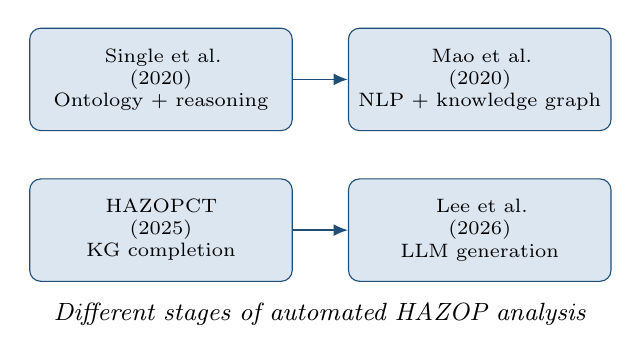
\begin{tikzpicture}[
    node distance=6mm and 7mm,
    box/.style={
        draw=hzblue,
        fill=hzbluebg,
        rounded corners,
        align=center,
        text width=31mm,
        minimum height=13mm,
        font=\scriptsize
    },
    arrow/.style={ar}
]

    \node[box] (single)
        {Single et al.\\(2020)\\
         Ontology + reasoning};

    \node[box, right=of single] (mao)
        {Mao et al.\\(2020)\\
         NLP + knowledge graph};

    \node[box, below=of single] (hazopct)
        {HAZOPCT\\(2025)\\
         KG completion};

    \node[box, right=of hazopct] (lee)
        {Lee et al.\\(2026)\\
         LLM generation};

    \node[below=8mm of $(hazopct)!0.5!(lee)$,
          align=center,
          text width=72mm,
          font=\small\itshape]
        (synthesis)
        {Different stages of automated HAZOP analysis};

    \draw[arrow] (single) -- (mao);
    \draw[arrow] (hazopct) -- (lee);

\end{tikzpicture}
\caption[Literature landscape for automated HAZOP analysis]
{The papers studied so far address different stages of automated HAZOP
analysis: structured symbolic reasoning, knowledge extraction and graph
construction, graph-based completion, and direct LLM-based generation.}
\label{fig:w3-literature-landscape}
\end{figure}

\section{A Layered View of the HAZOP Problem}

The comparison indicates that several capabilities must be distinguished when
discussing automated HAZOP analysis.

\begin{enumerate}
    \item \textbf{Information extraction:} identifying relevant entities,
    events, and relationships from documents.

    \item \textbf{Representation:} encoding extracted information using a
    structured representation such as a table, ontology, knowledge graph, or
    causal graph.

    \item \textbf{Causal reasoning:} determining how deviations, causes,
    effects, consequences, and safeguards are related and how events
    propagate through intermediate states.

    \item \textbf{Inference and validation:} identifying potentially missing
    relationships or scenarios and determining whether the resulting
    reasoning is consistent with process and safety knowledge.
\end{enumerate}

These capabilities are related but are not interchangeable. In particular,
identifying the concepts ``cooling failure'', ``high temperature'', and
``pressure increase'' does not by itself establish that they form an ordered
causal sequence.

The distinction is illustrated in Figure~\ref{fig:w3-layered-problem}.

\begin{figure}[htbp]
\centering
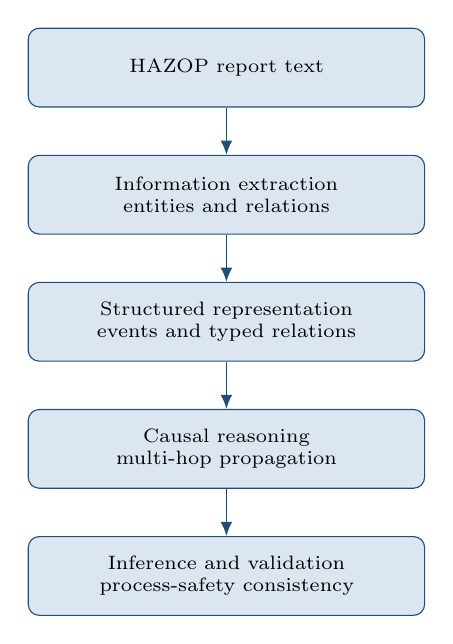
\begin{tikzpicture}[
    node distance=6mm,
    box/.style={
        draw=hzblue,
        fill=hzbluebg,
        rounded corners,
        align=center,
        text width=48mm,
        minimum height=10mm,
        font=\scriptsize
    },
    arrow/.style={ar}
]

    \node[box] (text)
        {HAZOP report text};

    \node[box, below=of text] (extract)
        {Information extraction\\
         entities and relations};

    \node[box, below=of extract] (repr)
        {Structured representation\\
         events and typed relations};

    \node[box, below=of repr] (reason)
        {Causal reasoning\\
         multi-hop propagation};

    \node[box, below=of reason] (valid)
        {Inference and validation\\
         process-safety consistency};

    \draw[arrow] (text) -- (extract);
    \draw[arrow] (extract) -- (repr);
    \draw[arrow] (repr) -- (reason);
    \draw[arrow] (reason) -- (valid);

\end{tikzpicture}
\caption[Layered view of automated HAZOP reasoning]
{A layered view of the HAZOP problem. Information extraction is an
intermediate step; causal reasoning additionally requires relationships,
direction, ordering, and propagation between events.}
\label{fig:w3-layered-problem}
\end{figure}

This distinction is particularly relevant to the present project. A system
may correctly identify individual HAZOP concepts while still failing to
recover the reasoning connecting those concepts.

\section{Why Causal Structure Is the Central Focus}

The literature studied so far suggests that the causal structure of HAZOP
information is more important than the presence of individual keywords alone.

Consider the following hypothetical description:

\begin{center}
\emph{Cooling-water failure may increase reactor temperature, which can cause
pressure buildup and ultimately result in loss of containment.}
\end{center}

A conventional information-extraction system may identify:

\begin{center}
\textit{cooling-water failure}, \quad
\textit{reactor temperature}, \quad
\textit{pressure buildup}, \quad
\textit{loss of containment}.
\end{center}

However, identifying these concepts does not establish the causal structure:

\begin{center}
\[
\text{Cooling failure}
\rightarrow
\text{Temperature increase}
\rightarrow
\text{Pressure increase}
\rightarrow
\text{Loss of containment}.
\]
\end{center}

The direction and ordering of these relationships are essential. A system
that detects all four concepts but assigns incorrect relationships has not
recovered the causal reasoning expressed by the original statement.

This distinction is also consistent with the progression of the literature.
Single et al.\ demonstrate that HAZOP reasoning can contain multi-step and
branching causal structures, while Mao et al.\ demonstrate how process-safety
information can be organized into a knowledge graph
\cite{single2020ontologyhazop,mao2020processsafetykg}.

The present investigation therefore focuses on the connection between
natural-language information and an explicit causal representation.

\section{Current Working Research Pipeline}

Based on the literature studied so far, the current working hypothesis is to
investigate a pipeline that begins with historical HAZOP reports rather than
with an already constructed process ontology.

The proposed high-level pipeline is:

\begin{center}
\emph{Historical HAZOP reports}
$\rightarrow$
\emph{NLP/LLM extraction}
$\rightarrow$
\emph{causal information}
$\rightarrow$
\emph{structured causal representation}
$\rightarrow$
\emph{causal reasoning}
$\rightarrow$
\emph{validation}.
\end{center}

Figure~\ref{fig:w3-working-pipeline} presents the same idea in a compact
system representation.

\begin{figure}[htbp]
\centering
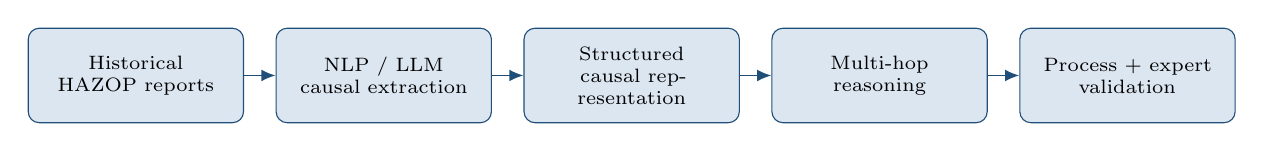
\begin{tikzpicture}[
    node distance=5mm and 4mm,
    box/.style={
        draw=hzblue,
        fill=hzbluebg,
        rounded corners,
        align=center,
        text width=25mm,
        minimum height=12mm,
        font=\scriptsize
    },
    arrow/.style={ar}
]

    \node[box] (reports)
        {Historical\\HAZOP reports};

    \node[box, right=of reports] (extract)
        {NLP / LLM\\
         causal extraction};

    \node[box, right=of extract] (graph)
        {Structured\\
         causal representation};

    \node[box, right=of graph] (reason)
        {Multi-hop\\
         reasoning};

    \node[box, right=of reason] (valid)
        {Process + expert\\
         validation};

    \draw[arrow] (reports) -- (extract);
    \draw[arrow] (extract) -- (graph);
    \draw[arrow] (graph) -- (reason);
    \draw[arrow] (reason) -- (valid);

\end{tikzpicture}
\caption[Current working research pipeline]
{Current working pipeline for investigating structured HAZOP reasoning from
historical reports. This is a working research hypothesis rather than a
finalized system architecture.}
\label{fig:w3-working-pipeline}
\end{figure}

The purpose of this pipeline is not to assume that a knowledge graph or a
particular ontology is already the correct representation. Instead, the
literature is being used to determine the representation and reasoning
requirements that the case study must satisfy.

In particular, the following questions remain open:

\begin{enumerate}
    \item Which HAZOP concepts need to be explicitly represented?

    \item Which relation types are required to distinguish causality from
    simple association?

    \item How should multi-step and branching causal chains be represented?

    \item How should multiple causes leading to a common effect be
    represented?

    \item How should safeguards be attached to causal chains?

    \item How should uncertainty in extracted relationships be represented?

    \item Can an extracted causal graph support reasoning over more than one
    causal hop?

    \item Can missing or incomplete causal relationships be identified?
\end{enumerate}

These questions will be used to define the case study and experimental
methodology in the subsequent sections of this week's report.

% ============================================================
% Week 03 --- Part II
% Case-study design and data requirements
% ============================================================

\section{Case-Study Design}

The literature review established that the central objective of this
research is not merely to identify HAZOP entities, but to recover the
causal structure connecting deviations, causes, consequences, and
safeguards. Therefore, the choice of case study is an important part of
the experimental design.

Rather than selecting a process solely because a HAZOP dataset is
available, the case study should provide sufficient causal structure
for evaluating information extraction and subsequent reasoning. The
selected process should also contain enough variation in terminology
and causal descriptions to test whether the proposed NLP/LLM approach
can generalize beyond a small collection of nearly identical sentences.

\subsection{Requirements for the Case Study}

The initial requirements for the case study are summarized in
Figure~\ref{fig:case-study-requirements}.

\begin{figure}[htbp]
\centering
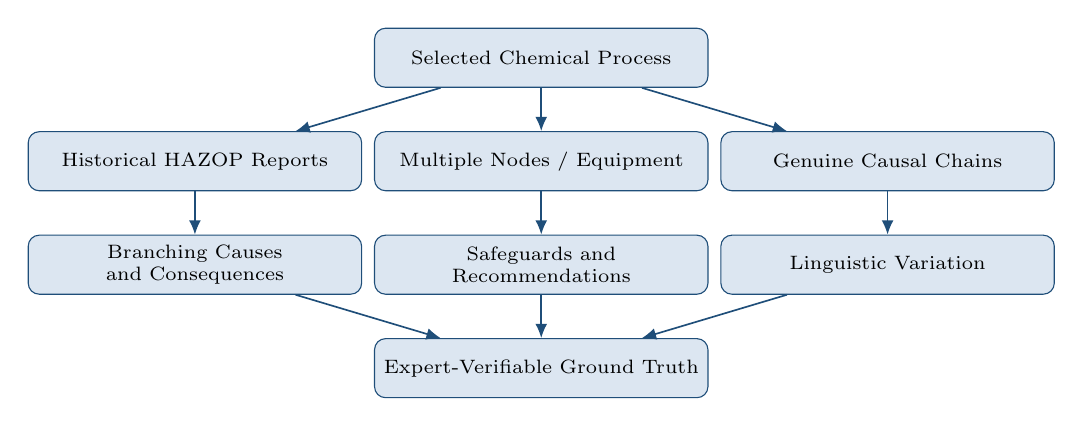
\begin{tikzpicture}[
    node distance=0.45cm,
    box/.style={
        rectangle,
        rounded corners,
        draw=hzblue,
        fill=hzbluebg,
        align=center,
        text width=4.0cm,
        minimum height=0.75cm,
        font=\scriptsize
    },
    arrow/.style={ar}
]

\node[box] (case) {Selected Chemical Process};

\node[box, below left=0.55cm and 0.15cm of case] (reports)
    {Historical HAZOP Reports};

\node[box, below=0.55cm of case] (nodes)
    {Multiple Nodes / Equipment};

\node[box, below right=0.55cm and 0.15cm of case] (chains)
    {Genuine Causal Chains};

\node[box, below=0.55cm of reports] (branch)
    {Branching Causes and Consequences};

\node[box, below=0.55cm of nodes] (safeguards)
    {Safeguards and Recommendations};

\node[box, below=0.55cm of chains] (variation)
    {Linguistic Variation};

\node[box, below=0.55cm of safeguards] (validation)
    {Expert-Verifiable Ground Truth};

\draw[arrow] (case) -- (reports);
\draw[arrow] (case) -- (nodes);
\draw[arrow] (case) -- (chains);

\draw[arrow] (reports) -- (branch);
\draw[arrow] (nodes) -- (safeguards);
\draw[arrow] (chains) -- (variation);

\draw[arrow] (branch) -- (validation);
\draw[arrow] (safeguards) -- (validation);
\draw[arrow] (variation) -- (validation);

\end{tikzpicture}
\caption{Initial requirements for selecting the case study.}
\label{fig:case-study-requirements}
\end{figure}

The following characteristics are considered desirable.

\begin{enumerate}[label=\textbf{\arabic*.}]

    \item \textbf{Availability of HAZOP reports:}
    The case study should have access to sufficiently detailed HAZOP
    worksheets or reports containing deviations, causes, consequences,
    safeguards, and relevant process context.

    \item \textbf{Multiple process nodes:}
    The process should contain multiple equipment items or HAZOP nodes
    so that the proposed method can be evaluated across different
    process contexts.

    \item \textbf{Explicit causal relationships:}
    The reports should contain statements from which causal
    relationships can be recovered rather than only isolated labels
    or keywords.

    \item \textbf{Multi-step causal chains:}
    The data should contain cases in which a cause produces an
    intermediate state or deviation that subsequently produces one or
    more consequences.

    \item \textbf{Branching structure:}
    Ideally, individual deviations should have multiple possible causes
    and consequences. This is important because a simple one-to-one
    mapping would not adequately test causal graph construction.

    \item \textbf{Safeguard information:}
    The HAZOP records should contain safeguards or recommendations so
    that the causal structure can eventually be connected to risk
    mitigation information.

    \item \textbf{Linguistic variation:}
    Different HAZOP entries should express similar causal relationships
    using different terminology or sentence structures. This allows
    the extraction system to be tested for semantic rather than
    purely lexical matching.

    \item \textbf{Expert-verifiable ground truth:}
    The extracted relationships and reconstructed causal chains should
    be capable of being checked against the original HAZOP analysis
    and, where possible, by a process-safety expert.

\end{enumerate}

\subsection{Why These Requirements Matter}

The requirements are motivated by the distinction between
information extraction and causal reasoning identified in the
literature.

For example, consider a simplified process-safety description:

\begin{center}
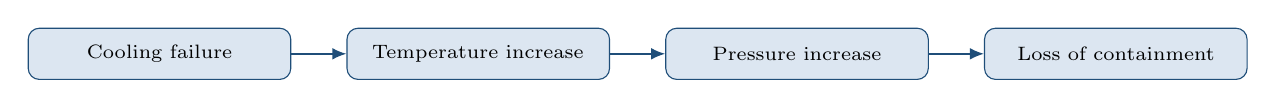
\begin{tikzpicture}[
    node distance=0.55cm,
    box/.style={
        rectangle,
        rounded corners,
        draw=hzblue,
        fill=hzbluebg,
        align=center,
        text width=3.1cm,
        minimum height=0.65cm,
        font=\scriptsize
    },
    arrow/.style={ar}
]

\node[box] (cause) {Cooling failure};
\node[box, right=0.7cm of cause] (temp) {Temperature increase};
\node[box, right=0.7cm of temp] (pressure) {Pressure increase};
\node[box, right=0.7cm of pressure] (loss) {Loss of containment};

\draw[arrow] (cause) -- (temp);
\draw[arrow] (temp) -- (pressure);
\draw[arrow] (pressure) -- (loss);

\end{tikzpicture}
\end{center}

In this example, identifying the four concepts is only the first
step. A useful system must also recover the relationships between
them. The resulting structure can be represented as

\begin{equation}
C_1 \rightarrow D_1 \rightarrow E_1 \rightarrow C_2,
\end{equation}

where the symbols represent successive causal states rather than
independent HAZOP entities.

Consequently, a case study containing only isolated statements such as
``high pressure'', ``valve failure'', or ``fire'' would be insufficient
for evaluating the main research objective. The dataset must contain
enough contextual information to determine how such concepts are
related.

\subsection{HAZOP Entry as the Basic Unit of Analysis}

The initial experimental unit will be an individual HAZOP entry or
worksheet row. A conventional entry can be viewed as containing
several semantically distinct components:

\begin{center}

\begin{tikzpicture}[
    node distance=0.45cm,
    box/.style={
        rectangle,
        rounded corners,
        draw=hzblue,
        fill=hzbluebg,
        align=center,
        text width=2.4cm,
        minimum height=0.65cm,
        font=\scriptsize
    },
    arrow/.style={ar}
]

\node[box] (node) {Node};
\node[box, right=0.35cm of node] (dev) {Deviation};
\node[box, right=0.35cm of dev] (cause) {Cause};
\node[box, right=0.35cm of cause] (effect) {Consequence};
\node[box, right=0.35cm of effect] (safe) {Safeguard};

\draw[arrow] (node) -- (dev);
\draw[arrow] (dev) -- (cause);
\draw[arrow] (cause) -- (effect);
\draw[arrow] (effect) -- (safe);

\end{tikzpicture}
\end{center}

This representation should not be interpreted as claiming that every
HAZOP entry forms a simple linear chain. Instead, it provides an
initial decomposition of the information contained in a worksheet.
The actual representation may contain multiple causes, intermediate
states, several consequences, and safeguards attached to different
parts of the causal structure.

\subsection{From HAZOP Rows to Causal Propositions}

A major objective of the case-study analysis will therefore be to
transform the textual information in a HAZOP entry into explicit
causal propositions.

For example, a textual entry could conceptually produce propositions
of the form

\begin{align}
\text{Cause} &\xrightarrow{\text{causes}} \text{Deviation},\\
\text{Deviation} &\xrightarrow{\text{leads\_to}} \text{Consequence},\\
\text{Consequence} &\xrightarrow{\text{mitigated\_by}} \text{Safeguard}.
\end{align}

The precise relation vocabulary is intentionally left open at this
stage. Determining whether these relations are sufficient, or whether
additional relations are required to represent intermediate process
states, is one of the questions to be investigated during the
subsequent design phase.

\subsection{Ground-Truth Construction}

The original HAZOP reports will serve as the primary source of
ground-truth information. However, the original worksheet structure
may not directly provide all of the intermediate causal links required
for evaluating multi-hop reasoning.

Therefore, the ground truth will be developed in stages:

\begin{enumerate}[label=\textbf{\arabic*.}]
    \item identify the relevant HAZOP entities in the source entry;
    \item identify explicitly stated causal relationships;
    \item identify multi-step relationships that are supported by the
    text and process context;
    \item represent alternative causes and consequences where they
    exist;
    \item associate safeguards with the corresponding causal scenario;
    \item obtain expert review for relationships that require process
    interpretation.
\end{enumerate}

This distinction is important because an automatically extracted graph
should not be treated as ground truth merely because the model
generated it. The reference structure must originate from the
available HAZOP evidence and, where necessary, expert assessment.

\subsection{Case-Study Selection Strategy}

At this stage, a specific process will not be selected solely on the
basis of convenience. Candidate datasets will instead be evaluated
against the requirements defined above.

The selection can be formulated as a screening process:

\begin{center}
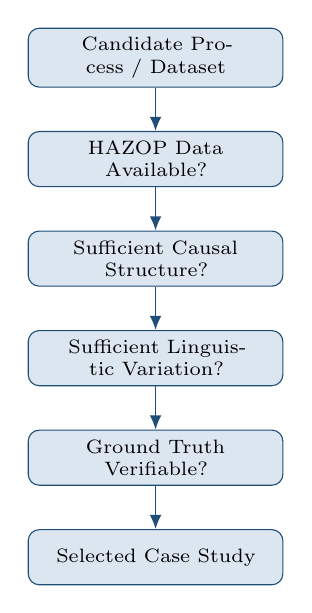
\begin{tikzpicture}[
    node distance=0.55cm,
    box/.style={
        rectangle,
        rounded corners,
        draw=hzblue,
        fill=hzbluebg,
        align=center,
        text width=3.0cm,
        minimum height=0.7cm,
        font=\scriptsize
    },
    arrow/.style={ar}
]

\node[box] (candidate) {Candidate Process / Dataset};

\node[box, below=0.55cm of candidate] (availability)
    {HAZOP Data Available?};

\node[box, below=0.55cm of availability] (structure)
    {Sufficient Causal Structure?};

\node[box, below=0.55cm of structure] (variation)
    {Sufficient Linguistic Variation?};

\node[box, below=0.55cm of variation] (validation)
    {Ground Truth Verifiable?};

\node[box, below=0.55cm of validation] (select)
    {Selected Case Study};

\draw[arrow] (candidate) -- (availability);
\draw[arrow] (availability) -- (structure);
\draw[arrow] (structure) -- (variation);
\draw[arrow] (variation) -- (validation);
\draw[arrow] (validation) -- (select);

\end{tikzpicture}
\end{center}

\subsection{Current Status}

The case-study process is therefore considered an open design
decision at this point. The immediate objective is to identify a
dataset that satisfies the causal and validation requirements rather
than to optimize for dataset size alone.

This approach also allows the research design to remain independent of
a particular process until the available HAZOP material has been
examined. Once candidate reports are obtained, their structure,
terminology, causal depth, branching, and available process context
can be compared against the requirements established in this section.

\subsection{Implications for the Experimental Design}

The case study will eventually support evaluation at several levels:

\begin{center}
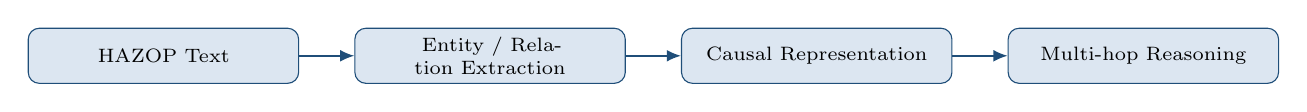
\begin{tikzpicture}[
    node distance=0.5cm,
    box/.style={
        rectangle,
        rounded corners,
        draw=hzblue,
        fill=hzbluebg,
        align=center,
        text width=3.2cm,
        minimum height=0.7cm,
        font=\scriptsize
    },
    arrow/.style={ar}
]

\node[box] (text) {HAZOP Text};
\node[box, right=0.7cm of text] (extract)
    {Entity / Relation Extraction};
\node[box, right=0.7cm of extract] (graph)
    {Causal Representation};
\node[box, right=0.7cm of graph] (reason)
    {Multi-hop Reasoning};

\draw[arrow] (text) -- (extract);
\draw[arrow] (extract) -- (graph);
\draw[arrow] (graph) -- (reason);

\end{tikzpicture}
\end{center}

This decomposition will make it possible to distinguish errors caused
by incorrect extraction from errors introduced during graph
construction or causal reasoning. Such separation is necessary for
determining whether an observed failure is an NLP problem, a
representation problem, or a reasoning problem.

The next stage of the research will therefore focus on examining
candidate HAZOP datasets and determining the exact causal schema that
can be reliably annotated from them.

% ============================================================
% Week 03 --- Part III
% Causal Schema, Experimental Design, and Next Steps
% ============================================================

\section{Causal Schema and Experimental Design}

The previous sections established the literature landscape and the
requirements for selecting a suitable HAZOP case study. The remaining
task is to define how the extracted information will be represented,
evaluated, and used for causal reasoning.

\subsection{Initial Causal Representation}

The working representation is based on typed entities and relationships
rather than the original tabular HAZOP format. The initial structure is:

\begin{center}
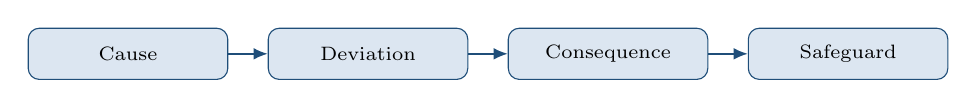
\begin{tikzpicture}[
    node distance=0.55cm,
    box/.style={
        rectangle,
        rounded corners,
        draw=hzblue,
        fill=hzbluebg,
        align=center,
        text width=2.3cm,
        minimum height=0.65cm,
        font=\scriptsize
    },
    arrow/.style={ar}
]

\node[box] (cause) {Cause};
\node[box, right=0.5cm of cause] (dev) {Deviation};
\node[box, right=0.5cm of dev] (cons) {Consequence};
\node[box, right=0.5cm of cons] (safe) {Safeguard};

\draw[arrow] (cause) -- (dev);
\draw[arrow] (dev) -- (cons);
\draw[arrow] (cons) -- (safe);

\end{tikzpicture}
\end{center}

This should not be interpreted as a restriction to linear chains. A
deviation may have multiple causes and consequences, while a
consequence may itself become an intermediate state in a longer causal
chain.

The representation can therefore be expressed as

\[
G=(V,E),
\]

where \(V\) contains entities and \(E\) contains typed relationships.

The initial entity types are:

\begin{center}
\begin{tabular}{ll}
\textbf{Entity} & \textbf{Description} \\
\hline
Process Node & HAZOP study location \\
Equipment & Physical equipment involved \\
Parameter & Process variable \\
Deviation & HAZOP deviation \\
Cause & Initiating or contributing condition \\
Consequence & Resulting outcome \\
Safeguard & Existing protective measure \\
Recommendation & Proposed protective action
\end{tabular}
\end{center}

The schema is provisional and will be revised after examination of the
selected HAZOP data.

\subsection{Causal Relations}

The initial relation vocabulary is:

\begin{center}
\begin{tabular}{ll}
\textbf{Relation} & \textbf{Meaning} \\
\hline
causes & Cause produces a deviation or state \\
leads\_to & One state produces another state or consequence \\
results\_in & Consequence relation \\
mitigated\_by & Protective measure associated with a scenario \\
associated\_with & Contextual association \\
has\_parameter & Equipment/node--parameter relationship \\
has\_deviation & Node--deviation relationship
\end{tabular}
\end{center}

The final relation vocabulary will be determined from the actual
language and causal structures present in the dataset.

\subsection{Annotation Strategy}

The basic annotation unit will be a causal proposition represented as

\[
(h,r,t),
\]

where \(h\) is the source entity, \(r\) is the relation, and \(t\) is
the target entity.

For example,

\[
(\text{Cooling Failure},\text{causes},\text{High Temperature})
\]

followed by

\[
(\text{High Temperature},\text{leads\_to},\text{Pressure Increase}).
\]

Multiple propositions can then be combined into a causal graph.

The annotation process will distinguish between:

\begin{enumerate}[label=\textbf{\arabic*.}]
    \item entities and process context;
    \item explicitly stated causal relationships;
    \item multi-step relationships;
    \item alternative causes and consequences;
    \item safeguards and recommendations.
\end{enumerate}

Implicit relationships that require substantial process interpretation
will be marked separately rather than automatically treated as
ground truth.

\subsection{Proposed Research Pipeline}

The complete working pipeline for the study is:

\begin{center}
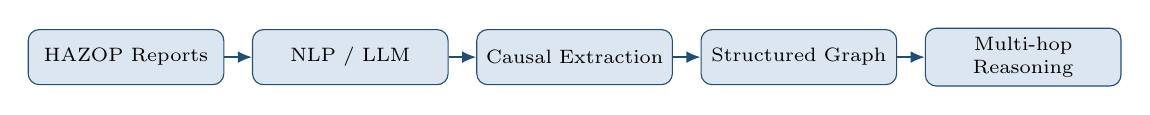
\begin{tikzpicture}[
    node distance=0.4cm,
    box/.style={
        rectangle,
        rounded corners,
        draw=hzblue,
        fill=hzbluebg,
        align=center,
        text width=2.25cm,
        minimum height=0.7cm,
        font=\scriptsize
    },
    arrow/.style={ar}
]

\node[box] (data) {HAZOP Reports};
\node[box, right=0.35cm of data] (extract) {NLP / LLM};
\node[box, right=0.35cm of extract] (causal) {Causal Extraction};
\node[box, right=0.35cm of causal] (graph) {Structured Graph};
\node[box, right=0.35cm of graph] (reason) {Multi-hop Reasoning};

\draw[arrow] (data) -- (extract);
\draw[arrow] (extract) -- (causal);
\draw[arrow] (causal) -- (graph);
\draw[arrow] (graph) -- (reason);

\end{tikzpicture}
\end{center}

The extracted structure will then be compared against the annotated
reference structure and evaluated for causal correctness.

\subsection{Experimental Comparison}

The initial experiments will compare different levels of extraction
and reasoning rather than evaluating only a single model.

\begin{description}[style=nextline,leftmargin=0pt,labelindent=0pt,font=\bfseries]

    \item[Experiment 1: Classical NLP baseline]

    A conventional pipeline using named entity recognition followed by
    relation extraction will provide a baseline for comparison.

    \item[Experiment 2: LLM structured extraction]

    An LLM will be prompted to extract HAZOP entities and typed causal
    relations into a predefined structured format.

    \item[Experiment 3: Explicit causal extraction]

    The extraction task will explicitly require identification of
    causal direction and intermediate states rather than simply
    identifying related entities.

    \item[Experiment 4: Causal graph reasoning]

    The extracted relations will be assembled into a graph and used
    for multi-hop reasoning.

    \item[Experiment 5: Missing-relation experiment]

    Known relationships can be temporarily removed from the graph and
    the system can be tested on whether it can recover the missing
    relationship or causal path.

\end{description}

The last experiment is particularly relevant to the distinction
between extraction and reasoning. A system that merely reproduces
information from the input is different from one that can use an
existing causal structure to identify a missing relationship.

\subsection{Evaluation Metrics}

Evaluation will be performed at multiple levels.

\begin{center}
\begin{tabular}{ll}
\textbf{Level} & \textbf{Possible Metrics} \\
\hline
Entity extraction & Precision, Recall, F1 \\
Relation extraction & Precision, Recall, F1 \\
Causal direction & Relation accuracy \\
Causal chains & Path Precision, Recall, F1 \\
Multi-hop reasoning & 1-hop / 2-hop / 3-hop accuracy \\
Missing relationships & Recovery accuracy, false positives \\
Safety validity & Expert/process-safety assessment
\end{tabular}
\end{center}

This separation is important because a system may achieve good entity
recognition while still producing incorrect causal relationships.

Similarly, correct relation extraction does not necessarily imply
successful multi-hop reasoning.

\subsection{Validation Strategy}

The final evaluation should therefore include both computational and
domain-based validation.

\begin{center}
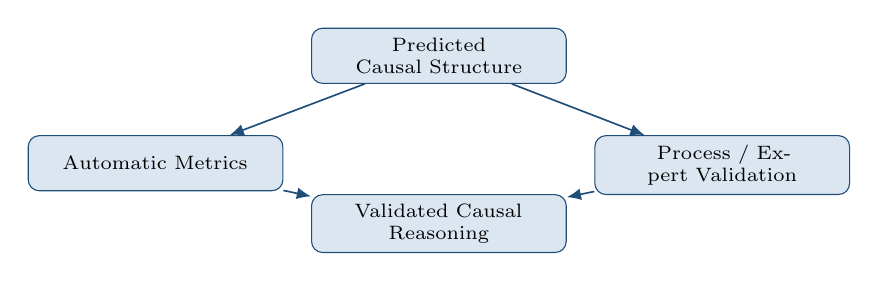
\begin{tikzpicture}[
    node distance=0.55cm,
    box/.style={
        rectangle,
        rounded corners,
        draw=hzblue,
        fill=hzbluebg,
        align=center,
        text width=3.0cm,
        minimum height=0.7cm,
        font=\scriptsize
    },
    arrow/.style={ar}
]

\node[box] (prediction) {Predicted Causal Structure};

\node[box, below left=0.65cm and 0.35cm of prediction]
    (metric) {Automatic Metrics};

\node[box, below right=0.65cm and 0.35cm of prediction]
    (expert) {Process / Expert Validation};

\node[box, below=1.4cm of prediction]
    (final) {Validated Causal Reasoning};

\draw[arrow] (prediction) -- (metric);
\draw[arrow] (prediction) -- (expert);
\draw[arrow] (metric) -- (final);
\draw[arrow] (expert) -- (final);

\end{tikzpicture}
\end{center}

Automatic metrics will measure agreement with the annotated reference
structure, while expert validation will be necessary for relationships
whose correctness depends on process knowledge or physical
interpretation.

\subsection{Working Research Question}

Based on the literature examined so far, the working research question
is:

\begin{quote}
\textit{Can natural-language processing and large language models
reliably extract the causal structure embedded in HAZOP reports and
represent it in a form that supports explicit multi-hop causal
reasoning?}
\end{quote}

This remains a working research question rather than a finalized claim
of novelty.

The investigation will focus on three supporting questions:

\begin{enumerate}
    \item Can NLP/LLMs reliably extract causal relationships from
    HAZOP text?

    \item Does an explicit causal representation improve multi-hop
    reasoning compared with direct generation of HAZOP conclusions?

    \item Can causal reasoning identify missing or overlooked
    relationships while maintaining process-safety validity?
\end{enumerate}

\subsection{Expected Research Direction}

The current understanding of the project can therefore be summarized
as:

\[
\boxed{\begin{gathered}
\text{Historical HAZOP Reports}\;\rightarrow\;\text{Causal Extraction}\;\rightarrow\\[-1pt]
\text{Structured Representation}\;\rightarrow\;\text{Multi-hop Reasoning}\;\rightarrow\;\text{Validation}
\end{gathered}}
\]

The specific representation---knowledge graph, ontology, causal graph,
or a hybrid approach---will not be fixed until the case-study data and
annotation requirements have been examined.

This preserves flexibility while keeping the central objective
unchanged: recovering and reasoning over the causal structure embedded
in HAZOP documentation.

\subsection{Next Steps}

The immediate next steps are:

\begin{enumerate}[label=\textbf{\arabic*.}]
    \item identify candidate HAZOP datasets;
    \item examine their structure and availability;
    \item select the case study using the requirements defined earlier;
    \item inspect representative HAZOP entries;
    \item refine the entity and relation schema;
    \item define the annotation format;
    \item construct an initial annotated subset;
    \item establish the first extraction baseline.
\end{enumerate}

These steps will provide the transition from literature and research
design into the implementation and experimental phase of the project.


% ------------------------------------------------------------
% Bibliography
% ------------------------------------------------------------
\small
\bibliographystyle{plain}
\bibliography{references}

\end{document}
